\documentclass[11pt]{article}
\usepackage[T1]{fontenc}
\usepackage{lmodern}
\usepackage[margin=1.1in]{geometry}
\usepackage{amsmath, amssymb, amsthm}
\usepackage{booktabs}
\usepackage{xcolor}
\definecolor{linknavy}{RGB}{25, 55, 125}
\usepackage[hypertexnames=false, colorlinks=true, linkcolor=linknavy, citecolor=linknavy, urlcolor=linknavy]{hyperref}
\hypersetup{
  pdftitle={The two 52-vertex counterexamples to the Petersen coloring conjecture are colorable only by themselves if no counterexample has at most 38 vertices},
  pdfauthor={Felipe Santibanez-Leal},
  pdfkeywords={Petersen coloring conjecture, H-coloring, cubic graphs, snarks, splitting lemma, SAT, DRAT}
}
\usepackage{orcidlink}
\usepackage{array}
\usepackage{placeins}
\usepackage{longtable}
\usepackage{algorithm}
\usepackage{algpseudocode}
\usepackage{tikz}
\usepackage{pgfplots}
\usepgfplotslibrary{groupplots}
\pgfplotsset{compat=1.17}
\usepackage{fancyhdr}

\newtheorem{theorem}{Theorem}[section]
\newtheorem{proposition}[theorem]{Proposition}
\newtheorem{lemma}[theorem]{Lemma}
\newtheorem{corollary}[theorem]{Corollary}
\theoremstyle{definition}
\newtheorem{definition}[theorem]{Definition}
\theoremstyle{remark}
\newtheorem{remark}[theorem]{Remark}

\newcommand{\PG}{P}
\newcommand{\Hthree}{\mathcal{H}_3}
\newcommand{\Ga}{G_{52}}
\newcommand{\Gb}{G'_{52}}
\newcommand{\Gsix}{G_{68}}
\newcommand{\Gmain}{G_{112}}
\newcommand{\Gsym}{H_{112}}
\newcommand{\evD}{\textnormal{[D]}}
\newcommand{\evMV}{\textnormal{[MV]}}
\newcommand{\evV}{\textnormal{[V]}}
\newcommand{\evU}{\textnormal{[U]}}
\algrenewcommand\algorithmicrequire{\textbf{Input:}}
\algrenewcommand\algorithmicensure{\textbf{Output:}}

\newcommand{\doctype}{Preprint}
\newcommand{\docversion}{v0.02}
\newcommand{\docdate}{14 November 2026}
\newcommand{\versiondoi}{10.5281/zenodo.22859075}
\newcommand{\conceptdoi}{10.5281/zenodo.22859074}
\newcommand{\docrepo}{github.com/fsantibanezleal/CAOS\_RESEARCH}
\newcommand{\headerblock}{%
\begin{center}
\fbox{\parbox{0.94\textwidth}{\small\raggedright
\textbf{\doctype} \quad$\cdot$\quad \docversion, \docdate \quad$\cdot$\quad Licence CC BY 4.0\\[2pt]
CAOS Research open-problems programme \quad$\cdot$\quad problem \texttt{petersen-coloring}\\[2pt]
Version DOI \href{https://doi.org/\versiondoi}{\texttt{\versiondoi}}\\[2pt]
Concept DOI (always latest) \href{https://doi.org/\conceptdoi}{\texttt{\conceptdoi}}\\[2pt]
Not peer reviewed. Source code, data and computational records: \href{https://\docrepo}{\texttt{\docrepo}}
}}
\end{center}
\vspace{4pt}}

\title{The Two 52-Vertex Counterexamples to the Petersen\\
Coloring Conjecture Are Colorable Only by Themselves\\
If No Counterexample Has at Most 38 Vertices}
\author{Felipe Santib\'a\~nez-Leal\,\orcidlink{0000-0002-0150-3246}\\
\small CAOS Research program, \texttt{github.com/fsantibanezleal/CAOS\_RESEARCH}}
\date{\docdate}

\pagestyle{fancy}
\fancyhf{}
\fancyhead[L]{\small CAOS Research \doctype}
\fancyhead[R]{\small Colorable Only by Themselves, Conditionally \textperiodcentered\ \docversion}
\fancyfoot[C]{\small \thepage}
\renewcommand{\headrulewidth}{0.4pt}
\fancypagestyle{plain}{\fancyhf{}\fancyfoot[C]{\small \thepage}\renewcommand{\headrulewidth}{0pt}}

\begin{document}
\maketitle
\headerblock

\begin{abstract}
For cubic graphs $G$ and $H$, an $H$-coloring of $G$ maps the edges of $G$ to the edges of $H$ so
that every vertex star of $G$ goes bijectively onto a vertex star of $H$; a Petersen coloring is the
case where $H$ is the Petersen graph. The graphs that no bridgeless cubic graph of smaller order
colors form the set $\mathcal{H}_3$ of Ma et al., infinite since the
conjecture was refuted in 2026. Goedgebeur et al.\ asked whether their 52-vertex
counterexamples are colorable only by themselves. We prove that the fibers of the vertex map of an
$H$-coloring have the same parity and that unused target vertices reduce to at most one; three kinds of
coloring remain, and the question becomes one propositional formula per target order, with the
target graph unknown. We prove the formula's symmetry breaking sound and certify each
refutation with a DRAT proof checked by \texttt{drat-trim}. For both counterexamples every even
target order from 40 to 50 is refuted; for the first one so are 2, 4 and 24 to 38. Assuming the
computation of the same authors, that no bridgeless cubic graph on at most 38 vertices
lacks a Petersen coloring, both graphs belong to $\mathcal{H}_3$. Without the two lemmas ten orders
of the first graph stayed undecided after 35 minutes; with them each took 137 to 5,882 seconds. Orders 6
to 22 of the first graph and 6 to 38 of the second remain undecided; 2 and 4 follow from 3-edge-colorability.
\end{abstract}


\section{Introduction}\label{sec:introduction}

\subsection{Colorings by a cubic graph}

Graphs are finite; they may have parallel edges but no loops. For a vertex $v$ of a graph $G$,
$\partial_G(v)$ is the set of edges at $v$. Let $G$ and $H$ be cubic graphs. An
\emph{$H$-coloring} of $G$ is a map $f : E(G) \to E(H)$ such that for every vertex $v$ of $G$
there is a vertex $u$ of $H$ with
\begin{equation}\label{eq:hcoloring}
f(\partial_G(v)) = \partial_H(u);
\end{equation}
since both stars have three edges, $f$ is injective on every star. If such a map exists we say that
$H$ \emph{colors} $G$. The relation is transitive. A \emph{Petersen coloring} is a $\PG$-coloring,
where $\PG$ is the Petersen graph, and a cubic graph is 3-edge-colorable if and only if it is colored
by the graph on two vertices with three parallel edges.

Jaeger~\cite{Jaeger1988} conjectured that every bridgeless cubic graph has a Petersen coloring.
The conjecture implies the Berge--Fulkerson conjecture and the 5-cycle double cover conjecture.
It was refuted in August 2026: Putman~\cite{Putman2026} gave two counterexamples $\Gmain$ and
$\Gsym$ on 112 vertices with computer-checked certificates, Jooken~\cite{Jooken2026} gave a proof that
can be checked by hand, and Goedgebeur, Jooken, M\'a\v{c}ajov\'a, Mattiolo, Mazzuoccolo and
Ulyanov~\cite{GJMMMU2026} gave two counterexamples $\Ga$ and $\Gb$ on 52 vertices with a purely
theoretical proof, cyclically 4-edge-connected counterexamples of every even order at least 60,
and the bounds $40 \le n_{\min} \le 52$ for the order $n_{\min}$ of a smallest counterexample. A
counterexample $\Gsix$ on 68 vertices is also available from the House of
Graphs~\cite{HoG}.

\subsection{The set \texorpdfstring{$\Hthree$}{H3} and the question}

Ma, Mattiolo, Steffen and Wolf~\cite{MMSW2025} proved that there is a unique inclusion-wise
minimal set $\Hthree$ of connected bridgeless cubic graphs such that every connected bridgeless
cubic graph is colored by a member of $\Hthree$, and they characterized its members
(Theorem~\ref{thm:mmsw}). The Petersen coloring conjecture was the statement $\Hthree = \{\PG\}$.
By~\cite{MMSW2025}, $\Hthree$ is either $\{\PG\}$ or infinite, so it is now known to be infinite, and
its members other than $\PG$ are all counterexamples: if $H$ colors a counterexample $G$ then $H$ is
a counterexample, because a Petersen coloring of $H$ composed with the $H$-coloring of $G$ would be
a Petersen coloring of $G$. In particular a smallest counterexample belongs to $\Hthree$.
Goedgebeur et al.\ ask~\cite[Section~5.4]{GJMMMU2026} whether their counterexamples of order 52
are colorable only by themselves, and observe that the question is tied to whether these graphs
are smallest counterexamples.

The question has two informative answers. A bridgeless cubic graph of order less than 52 that
colors $\Ga$ or $\Gb$ would be a counterexample below the known upper bound. If no such graph
exists, the 52-vertex graph is a member of $\Hthree$. Deciding it is a search over every cubic graph
of every even order below 52, with the target graph unknown, so no fixed instance of a satisfiability
problem states it. The difficulty is that a naive encoding leaves part of the unknown target
unconstrained by $G$, and a solver then enumerates completions of that free part without converging in the time available
(Section~\ref{sec:ablation}).

\subsection{Contributions and main result}

The contributions are the following; the marks \evD, \evMV, \evV{} and \evU{} that qualify the
statements are defined in Section~\ref{sec:problem}.
\begin{enumerate}
\item Two lemmas on the vertex map of an $H$-coloring (Section~\ref{sec:fibers}). All fibers have the same
parity (Lemma~\ref{lem:parity}), and unused target vertices can be reduced to at most one by the splitting
lemma (Lemma~\ref{lem:unused}). They leave three kinds of colorings (Corollary~\ref{cor:modes}) and turn
the question into finitely many propositional formulas, one per target order, whose unknown target has
no part left free. Two small consequences are proved as well: the extreme order $n-2$ and the orders 2
and 4 (Propositions~\ref{prop:nminus2} and~\ref{prop:small}).
\item The formula itself, stated in full (Section~\ref{sec:method}): every variable and clause family with its
count as a function of the order $n$ of $G$ and the target order $k$, a symmetry breaking with a soundness
proof, and a family of static clauses that is shown to be implied by the others
(Section~\ref{sec:theory}).
\item A certification pipeline (Algorithm~\ref{alg:certify}) with its parameters, tools and commands: every
unsatisfiable answer is a DRAT proof of the formula that is written to disk, hashed and checked by
\texttt{drat-trim}; every satisfiable answer is checked from the definition by a separate program.
\item Refutations for the three graphs. For both 52-vertex counterexamples every even target order from 40
to 50 is refuted; for the first one so are 2, 4 and 24 to 38 (Theorem~\ref{thm:orders},
Table~\ref{tab:orders}); for the 68-vertex graph the orders 62, 64 and 66 are refuted.
\item A conditional membership result: assuming Observation~10 of~\cite{GJMMMU2026}, both 52-vertex
graphs are colorable only by themselves (Theorem~\ref{thm:h3}).
\item The validation: 21 control instances on which the formulas with and without the fiber constraints
agree, and a measured ablation of the constraints (Sections~\ref{sec:results} and~\ref{sec:ablation}).
\item A complete record of the orders that remain undecided and why (Table~\ref{tab:undecided}).
\end{enumerate}

The main result is Theorem~\ref{thm:h3}: assuming the exhaustive computation of
Goedgebeur et al.\ that no bridgeless cubic graph on at most 38 vertices lacks a Petersen coloring,
$\Ga$ and $\Gb$ belong to $\Hthree$. The part of the proof that is new, Theorem~\ref{thm:orders}, does not
depend on that computation. The paper is organized as follows. Section~\ref{sec:related} places the work
among the published results. Section~\ref{sec:problem} fixes the definitions, the notation and the evidence
marks. Section~\ref{sec:fibers} proves the reduction lemmas, Section~\ref{sec:method} describes the formula
and the pipeline, and Section~\ref{sec:theory} proves them correct. Sections~\ref{sec:design} to~\ref{sec:ablation}
describe the experiments, the results and the ablation; Sections~\ref{sec:discussion} to~\ref{sec:conclusions} discuss
them, state their limits and conclude.

\section{Related work}\label{sec:related}

\paragraph{The conjecture and its refutation.} Jaeger stated the conjecture in 1988~\cite{Jaeger1988}
\evU{}; the 1988 chapter was not read here and is cited as every recent source cites it. Jaeger also showed
that a cubic graph has a Petersen coloring exactly when it has a normal 5-edge-coloring~\cite{Jaeger1985}
\evU{}, a form proved bijectively in~\cite[Proposition~2.1]{Putman2026} \evV{}; Mazzuoccolo and
Mkrtchyan study normal edge-colorings~\cite{MazzuoccoloMkrtchyan2020} \evV{} (abstract) and normal
6-edge-colorings~\cite{MazzuoccoloMkrtchyan2020b} \evU{}. The refutation is the work of three groups.
Putman's two 112-vertex counterexamples carry computer-checked certificates~\cite{Putman2026}
\evV{}. Jooken's note~\cite{Jooken2026} \evV{} isolates the mechanism by which a small subgraph forces four
pairwise adjacent edges of the Petersen graph. The group of Goedgebeur, Jooken, M\'a\v{c}ajov\'a,
Mattiolo, Mazzuoccolo and Ulyanov first gave the two 52-vertex graphs~\cite{GJMMM2026zenodo} \evV{}, and in the
final paper~\cite{GJMMMU2026} \evV{} added the infinite family of Theorem~8 there, the bounds
$40 \le n_{\min} \le 52$, the House of Graphs entries 57244 and 57278 for the 52-vertex graphs, and Section~5.4, the question this paper answers conditionally. The searches of 6 October 2026
found no later work on the conjecture or its counterexamples \evU{}, and that final paper still poses the question.

\paragraph{Colorings by a cubic graph and universal families.} Ma, Mattiolo, Steffen and
Wolf~\cite{MMSW2025} \evV{} define $H$-colorings between $r$-graphs, prove that the minimal universal set
$\mathcal{H}_r$ is unique (Corollary~3.8 there) and characterize its members (Theorem~3.7); Theorem~3.4 shows
that a class 2 $r$-graph not colored by any smaller $r$-graph is colored only by itself, and Observation~3.1 that an
$H$-coloring pulls back disjoint perfect matchings. Putman~\cite{Putman2026} \evV{} used their results to
conclude that one counterexample yields infinitely many. Ma, Steffen, Wolf and Zhang~\cite{MaSWZ2024}
\evU{} treat perfect-matching conjectures for $r$-graphs; the literature search found in it no statement on
the membership of a graph in $\mathcal{H}_r$. The question of this paper is thus a question about membership in
$\mathcal{H}_3$ for a specific graph, which no published result decides.

\paragraph{Colorings by specific targets.} The Petersen graph is the best-studied target. Kardo\v{s},
M\'a\v{c}ajov\'a and Zerafa~\cite{KardosMZ} showed, as reported in~\cite[Section~5.4]{GJMMMU2026}, that the Petersen graph is
colored only by itself or by graphs with a bridge \evU{}; the formula of this paper uses the statement as a control.
H\"agglund and Steffen study Petersen colorings of families of snarks~\cite{HagglundSteffen2014} \evU{}. Sylvester
colorings, that is, colorings by the graphs $S_{10}$ and $S_{12}$, are studied by Ferrarini and
Mkrtchyan~\cite{FerrariniMkrtchyan2026} \evU{}, and a counterexample to the conjectures on them is announced
in~\cite{S10S12counter} \evU{}. The revision arXiv:2608.10028v4~\cite{GJMMMU2026} presents a Petersen
coloring as a cycle-continuous map to the Petersen graph (DeVos, Ne\v{s}et\v{r}il and Raspaud~\cite{DeVosNR}) and links the problem to
matroids and to zero-temperature states of spin models \evV{}; it cites
Inoue et al.~\cite{InoueEtAl2026} \evU{} on 3-edge-colorings of apex cubic graphs. None of these works tests, for
a given graph, every cubic target of a given order at once; the target is fixed in each of them.

\paragraph{Verification frontier for small counterexamples.} Brinkmann, Goedgebeur, H\"agglund and
Markstr\"om generated all snarks on at most 36 vertices and observed that the conjecture holds for them~\cite{Brinkmann2013}
\evV{} (abstract). Goedgebeur, M\'a\v{c}ajov\'a and \v{S}koviera completed the order-36 case for weak snarks of girth 4
\cite{GMS2019}, as reported in~\cite{GJMMMU2026} \evU{}, so that no counterexample has at most 36 vertices. The lower bound 40 of~\cite{GJMMMU2026} comes
from an exhaustive check of the weak snarks on 38 vertices, a list of 7,142,217,899 graphs that took about 12 CPU-years
(Brinkmann and Van Overberghe's list~\cite{BrinkmannVO}, as cited there) \evV{}; that computation is not reproduced here.

\paragraph{Satisfiability and proof certification.} The refutations of the 52-vertex graphs by Petersen colorings
and by normal 5-edge-colorings are reproduced independently in Section~\ref{sec:results} with the programme's own edge-map and normal-coloring
encodings, independent of those of~\cite{Putman2026}. The solver is CaDiCaL~\cite{CaDiCaL} and the proof checker is
\texttt{drat-trim}~\cite{DRATtrim}; the splitting lemma behind Lemma~\ref{lem:unused} is Fleischner's~\cite{Fleischner1992} \evU{} in the
bridgeless form of Kaiser, Ku\v{z}el, Li and Wang~\cite{KaiserKLW2007} \evV{}. Open Problem Garden~\cite{OPG} \evV{} lists the conjecture and its
consequences.

\paragraph{Where this work stands.} Computational work on the conjecture decides whether one given graph has a
Petersen coloring, with the target fixed. The present work decides whether any cubic graph of a given order colors a given
graph, with the target as part of the unknown, and it does so with certificates for every refutation. Its two mathematical
ingredients, the parity of the fibers and the reduction of unused vertices, are what make the unknown target finite
and constrained everywhere; its limits are the external computation on which membership in $\Hthree$ rests and the orders
that no solver decided (Section~\ref{sec:limitations}).

\section{Problem formulation}\label{sec:problem}

\paragraph{Definitions.} Let $G$ be a connected cubic graph of order $n$ and $H$ a connected cubic graph.
An $H$-coloring $f$ of $G$ (Equation~\eqref{eq:hcoloring}) has a \emph{vertex map} $\varphi : V(G) \to V(H)$,
a map with $f(\partial_G(v)) = \partial_H(\varphi(v))$ for every $v$. A vertex map exists by definition, and it is
unique unless $H$ is the graph with two vertices and three parallel edges. The \emph{fiber} of $x \in V(H)$
is $\varphi^{-1}(x)$, of size $n_x$; the vertex $x$ is \emph{used} if $n_x > 0$, and $U$ and $W = V(H) \setminus U$
are the sets of used and unused vertices. A graph is \emph{bridgeless} if deleting any one edge leaves the number of its components unchanged;
Theorem~\ref{thm:mmsw} is stated for connected bridgeless cubic graphs.

\begin{theorem}[\cite{MMSW2025}, Theorem~3.7, case $r = 3$; \evV]\label{thm:mmsw}
For a connected bridgeless cubic graph $G$ the following are equivalent: $G \in \Hthree$; the only
connected bridgeless cubic graph that colors $G$ is $G$ itself; no bridgeless cubic graph of
smaller order colors $G$.
\end{theorem}

The implication from the third statement to the second is Theorem~3.4 there and holds for graphs of class 2, which $\Ga$, $\Gb$ and $\Gsix$ are (none is 3-edge-colorable). A disconnected bridgeless graph that colors the connected graph $G$ has a component that colors it, so asking for a connected colorer loses nothing.

\paragraph{The decision problem.} For a graph $G$ of order $n$, the question of~\cite[Section~5.4]{GJMMMU2026} is
whether some connected bridgeless cubic graph of order less than $n$ colors $G$. By Theorem~\ref{thm:mmsw} the answer is no
if and only if $G \in \Hthree$. The computational problem solved in this paper is a relaxation of it that
can be decided one target order at a time: given $G$ and an even $k < n$, does there exist a loopless cubic graph $H$
on $k$ vertices, connected or not and bridgeless or not, with an $H$-coloring of $G$ whose vertex map is of one of the
three kinds of Corollary~\ref{cor:modes}? Section~\ref{sec:fibers} shows that the union of these problems over all even
$k < n$ answers the question of Goedgebeur et al.; a refutation for a given $k$ is unconditional on connectedness
because the relaxed problem has more solutions.

\paragraph{Assumptions and their sources.} Graphs are finite and may have parallel edges but no loops, as in~\cite{MMSW2025};
the graphs $\Ga$, $\Gb$ and $\Gsix$ are simple, cubic, of girth 5, with edge connectivity 3 and cyclically 4-edge-connected
\evMV{}, and their edge lists are the House of Graphs entries 57244, 57278 and 57280 ($\Ga$ was checked isomorphic to the graph
printed in the first public version of~\cite{GJMMM2026zenodo}). The only external result used is Observation~10
of~\cite{GJMMMU2026} \evV{}, whose statement we use in the form: every bridgeless cubic graph with at most 38 vertices
has a Petersen coloring (equivalently, a smallest counterexample has at least 40 vertices, since cubic graphs have even order).

\paragraph{Evidence marks.} Every statement carries one of four marks. \evD{} marks a statement derived here with a proof in
the text. \evMV{} marks a statement machine-verified: a satisfiable answer accepted by the independent checker, or an unsatisfiable
answer whose DRAT proof \texttt{drat-trim} verified. \evV{} marks a statement read in the primary source cited. \evU{} marks a
statement known only through another source or not checked. A mark in a theorem header qualifies the whole statement; a theorem
that depends on an external statement carries both marks, and states the dependence in its hypothesis.

\begin{table}[t]\centering\small
\begin{tabular}{lp{0.74\textwidth}}
\toprule
symbol & meaning \\
\midrule
$G$, $n$ & connected cubic graph to be colored and its order; $\Ga$, $\Gb$, $\Gsix$ are the 52-, 52- and 68-vertex counterexamples \\
$H$, $k$ & target graph (loopless, cubic) and its order, an even number below $n$ \\
$f$, $\varphi$ & the $H$-coloring $E(G) \to E(H)$ and its vertex map $V(G) \to V(H)$ \\
$n_x$, $U$, $W$ & size of the fiber of $x$, the used and the unused target vertices \\
$\partial_G(v)$ & the three edges at $v$, in a fixed order $r = 0, 1, 2$ (the incidence order) \\
$(i,s)$ & slot $s \in \{0,1,2\}$ of target vertex $i < k$: one end of an edge of $H$ \\
$x_{v,i}$, $z_{v,r,s}$, $p_{a,b}$ & vertex $v$ goes to target $i$; the $r$-th edge at $v$ goes to slot $s$; slots $a$, $b$ are matched \\
$w_{v,r,i,s}$, $u_{v,i}$, $q$ & $x_{v,i} \wedge z_{v,r,s}$; target $i$ is used by a vertex $\le v$; all fibers are odd \\
$\mathcal{H}_3$ & the unique minimal set of connected bridgeless cubic graphs coloring every one \\
\bottomrule
\end{tabular}
\caption{Notation of Sections~\ref{sec:fibers} to~\ref{sec:theory}: graph symbols, the variables of the formula and their meaning, and the
mathematical objects they stand for. Slots are the three ends of the edges at a target vertex; the matching on them is the unknown target graph.}\label{tab:notation}
\end{table}

Table~\ref{tab:notation} collects the symbols. Slots and the matching $p$ carry the target graph in the formula: a perfect matching on the $3k$ slots that
never pairs two slots of the same vertex is the edge set of a loopless cubic graph on $k$ vertices, and every such graph arises from some matching,
so the unknown graph $H$ is encoded by $\binom{3k}{2} - 3k$ Boolean variables.

\section{Fibers of an \texorpdfstring{$H$}{H}-coloring: the reduction}\label{sec:fibers}

Throughout this section $G$ is a connected cubic graph of order $n$, $H$ is a connected cubic graph, $f$ is an
$H$-coloring of $G$, and $\varphi : V(G) \to V(H)$ is a vertex map of $f$, with the notation of
Section~\ref{sec:problem}. The two lemmas below are the mathematical core of the method: they show that the
vertices of the unknown target are of three kinds only, and that none of them is free.

\begin{lemma}[fiber parity; \evD]\label{lem:parity}
For every edge $e = xy$ of $H$, the set $f^{-1}(e)$ is a perfect matching of the subgraph of $G$
induced on $\varphi^{-1}(x) \cup \varphi^{-1}(y)$. Consequently
\begin{equation}\label{eq:parity}
|f^{-1}(e)| = \tfrac12\,(n_x + n_y),
\end{equation}
$n_x + n_y$ is even for every edge $xy$ of $H$, and all the numbers $n_x$, $x \in V(H)$, have the same parity.
\end{lemma}

\begin{proof}
A vertex $v$ of $G$ is incident with an edge of $f^{-1}(e)$ if and only if
$e \in f(\partial_G(v)) = \partial_H(\varphi(v))$, that is, if and only if
$\varphi(v) \in \{x, y\}$. In that case it is incident with exactly one such edge, because $f$ is
injective on $\partial_G(v)$. Hence $f^{-1}(e)$ is a matching that covers exactly
$\varphi^{-1}(x) \cup \varphi^{-1}(y)$, a set of $n_x + n_y$ vertices. The last statement follows
because $H$ is connected.
\end{proof}

So an $H$-coloring is of one of two kinds. If the fibers are odd, every vertex of $H$ is used and
$|V(H)| \le n$. If the fibers are even, at most $n/2$ vertices of $H$ are used. Both kinds occur:
an isomorphism has fibers of size~1, and a 3-edge-coloring of a graph of order $n \equiv 0
\pmod 4$ has a vertex map with two fibers of size $n/2$. Figure~\ref{fig:fibers} shows all three kinds that
appear below on one example, the complete graph on four vertices colored by the graph with two vertices and three
parallel edges.

\tikzset{ca/.style={circle,draw,fill=black,inner sep=1.7pt}, cb/.style={circle,draw,fill=white,line width=0.8pt,inner sep=1.7pt},
  cu/.style={circle,draw,dashed,fill=white,inner sep=1.7pt},
  m1/.style={line width=1.1pt}, m2/.style={dashed,line width=0.8pt}, m3/.style={dotted,line width=1.3pt}}
\newcommand{\kfour}[4]{%
\begin{tikzpicture}[solid,scale=0.85]
\node[#1] (a) at (0,1.2) {}; \node[#2] (b) at (1.2,1.2) {}; \node[#3] (c) at (1.2,0) {}; \node[#4] (d) at (0,0) {};
\draw[m1] (a)--(b); \draw[m1] (c)--(d);
\draw[m2] (b)--(c); \draw[m2] (d)--(a);
\draw[m3] (a)--(c); \draw[m3] (b)--(d);
\end{tikzpicture}}
\newcommand{\tgt}[2]{%
\begin{tikzpicture}[solid,scale=0.85]
\node[#1] (x) at (0,0) {}; \node[#2] (y) at (1.6,0) {};
\draw[m1] (x) to[bend left=35] (y); \draw[m2] (x) -- (y); \draw[m3] (x) to[bend right=35] (y);
\end{tikzpicture}}
\begin{figure}[t]
\centering
\begin{minipage}[t]{0.31\textwidth}\centering \kfour{ca}{cb}{cb}{cb}\\[4pt] \tgt{ca}{cb}\\[2pt] {\small (O) fibers $1, 3$}\end{minipage}\hfill
\begin{minipage}[t]{0.31\textwidth}\centering \kfour{ca}{ca}{cb}{cb}\\[4pt] \tgt{ca}{cb}\\[2pt] {\small (E0) fibers $2, 2$}\end{minipage}\hfill
\begin{minipage}[t]{0.31\textwidth}\centering \kfour{ca}{ca}{ca}{ca}\\[4pt] \tgt{ca}{cu}\\[2pt] {\small (E1) fibers $4, 0$}\end{minipage}
\caption{The three kinds of vertex maps on one example. The graph $K_4$ (top; the three perfect matchings are drawn solid, dashed and dotted) is colored by the graph with two vertices and three parallel edges (bottom) by sending each matching to one edge. Both target vertices have the same star, so every map from the four vertices to the two targets is a vertex map: fibers of sizes 1 and 3 are kind (O), sizes 2 and 2 kind (E0), and sizes 4 and 0 kind (E1), with an unused target drawn dashed.}\label{fig:fibers}
\end{figure}


The second lemma concerns the vertices of $H$ that are not used. We use the splitting lemma of
Fleischner~\cite{Fleischner1992} in the following form. Let $v$ be a vertex of a graph $K$ and
$e_1 = vv_1$, $e_2 = vv_2$ two edges at $v$. \emph{Splitting $e_1$ and $e_2$ off $v$} means adding
a new vertex $v^*$ and replacing $e_1, e_2$ by edges $v^*v_1$, $v^*v_2$.

\begin{lemma}[\cite{KaiserKLW2007}, Lemma~1, a consequence of~\cite{Fleischner1992}; \evV]\label{lem:split}
Let $v$ be a vertex of degree at least~4 in a bridgeless graph $K$. There exist edges $e_1, e_2$
incident with $v$ such that the graph obtained by splitting $e_1$ and $e_2$ off $v$ is bridgeless.
\end{lemma}

\begin{lemma}[unused vertices; \evD]\label{lem:unused}
Let $H$ be bridgeless and suppose $W \ne \emptyset$. Let $m$ be the number of edges between $U$
and $W$. Then there is a connected bridgeless cubic graph $H'$ with vertex set $U \cup W'$, where
$W' = \emptyset$ if $m$ is even and $|W'| = 1$ if $m$ is odd, and an $H'$-coloring of $G$ with
the same vertex map $\varphi$. In particular $|V(H')| \le |V(H)|$.
\end{lemma}

\begin{proof}
Every edge of $H$ with an end in $U$ lies in the image of $f$, since the star of a used vertex is
the image of a star of $G$; no edge with both ends in $W$ does. Identify $W$ to a single vertex
$w^*$ and delete the loops that arise. Every edge cut of the resulting graph $H_1$ is an edge cut
of $H$, so $H_1$ is bridgeless; $w^*$ has degree $m$, and $m \ge 2$ because $H$ is connected and
bridgeless. Every other vertex of $H_1$ is a used vertex, of degree~3, with its star unchanged.

While $w^*$ has degree at least~4, apply Lemma~\ref{lem:split} to split two edges $aw^*$, $bw^*$
off $w^*$ so that the graph stays bridgeless. Then $a \ne b$: otherwise the new vertex would be
joined to the cubic vertex $a$ by two parallel edges, and the third edge at $a$ would be a bridge.
Suppress the new vertex, that is, replace its two edges by a single edge $ab$. This keeps the graph
loopless and bridgeless and lowers the degree of $w^*$ by~2. When the degree of $w^*$ has dropped
to~3, stop. When it has dropped to~2, suppress $w^*$ in the same way; its two neighbours are
distinct by the same argument. Let $H'$ be the final graph. It is cubic, loopless and bridgeless.

Let $\mu$ map every edge of $H$ that has an end in $U$ to the edge of $H'$ that contains it. Two
edges merged in one step have their ends other than $w^*$ at distinct vertices, so $\mu$ is
injective on $\partial_H(u)$ and $\partial_{H'}(u) = \mu(\partial_H(u))$ for every $u \in U$. Hence
$\mu \circ f$ is an $H'$-coloring of $G$ with vertex map $\varphi$.

Finally $H'$ is connected. If $uv$ is an edge of $G$ with $\varphi(u) \ne \varphi(v)$, then
$f(uv)$ joins $\varphi(u)$ to $\varphi(v)$; it has both ends in $U$ and is therefore an edge of
$H'$. As $G$ is connected, $U$ induces a connected subgraph of $H'$, and the vertex $w^*$, if it
remains, is joined to $U$.
\end{proof}

Lemma~\ref{lem:unused} is the step that removes the free part of the target. A vertex of $H$ that no vertex of $G$
uses is joined to the rest of $H$ by edges that no edge of $G$ is mapped to, so a solver that searches for $H$ may place
there any bridgeless completion, and each completion is a different model. The lemma shows that nothing is lost by
asking for at most one such vertex, and the parity statement of Lemma~\ref{lem:parity} decides, from the order alone, whether
that vertex can exist.

\begin{corollary}[\evD]\label{cor:modes}
A connected cubic graph $G$ of order $n$ is colored by a connected bridgeless cubic graph of order
less than $n$ if and only if, for some even $k < n$, it has an $H$-coloring by a connected
bridgeless cubic graph $H$ of order $k$ with a vertex map of one of the following kinds:
\begin{enumerate}
\item[\textup{(O)}] every vertex of $H$ is used and every fiber is odd;
\item[\textup{(E0)}] every vertex of $H$ is used and every fiber is even, so that $k \le n/2$;
\item[\textup{(E1)}] exactly one vertex of $H$ is not used and every other fiber is even and
nonempty, so that $k - 1 \le n/2$.
\end{enumerate}
\end{corollary}

\begin{proof}
Let $H$ of order less than $n$ color $G$. If every vertex of $H$ is used, Lemma~\ref{lem:parity}
gives (O) or (E0). Otherwise the fibers are even by Lemma~\ref{lem:parity}, since an unused vertex
has an empty fiber, and Lemma~\ref{lem:unused} gives a graph $H'$ of order at most $|V(H)|$ with
the same vertex map and at most one unused vertex, which is (E0) or (E1).
\end{proof}

The kinds (O), (E0), (E1) leave no part of $H$ unconstrained by $G$: every edge of $H$ is the image
of an edge of $G$. For $n = 52$ the kind (O) is possible for every even order $k \le 50$, while (E0) and
(E1) require $k \le n/2 = 26$ and $k - 1 \le 26$, so they occur only for $k \le 26$; in the kind (O) with $k = 50$
the fibers are forty-nine singletons and one fiber of size three. For target orders close to $n$ only kind (O) is possible, and the fibers are then
almost all singletons. The extreme case of kind (O) can be settled by hand.

\begin{proposition}[\evD]\label{prop:nminus2}
Let $G$ be a connected simple cubic graph of order $n \ge 8$ without triangles. Then $G$ has no
$H$-coloring by a connected cubic graph $H$ of order $n - 2$ in which every vertex of $H$ is used.
\end{proposition}

\begin{proof}
Since $n - 2 > n/2$ and every vertex of $H$ is used, the fibers are odd by
Lemma~\ref{lem:parity}; hence one fiber $\{u_1, u_2, u_3\} = \varphi^{-1}(x)$ has size~3 and all
others have size~1. For each of the three edges $e = xy$ at $x$, the set $f^{-1}(e)$ is a perfect matching on
$\{u_1, u_2, u_3\}$ together with the single vertex of the fiber of $y$
(Lemma~\ref{lem:parity}), so it contains an edge of $G$ joining two of $u_1, u_2, u_3$. The three
sets $f^{-1}(e)$ are pairwise disjoint and $G$ is simple, so $u_1u_2u_3$ is a triangle of $G$.
\end{proof}

The hypothesis \emph{simple} is used in the last step: with parallel edges, two of the three disjoint sets could join the
same pair of vertices of the fiber. The flower snark $J_3$, which has triangles, is colored by a graph of order $n - 2 = 10$ with
one fiber of size three and nine singletons (Table~\ref{tab:controls}), so the triangle hypothesis cannot be dropped.

The smallest target orders follow from the 3-edge-colorability of the targets alone.

\begin{proposition}[\evD]\label{prop:small}
Let $G$ be a connected cubic graph that is not 3-edge-colorable. No loopless cubic graph on 2 or on 4 vertices colors $G$.
\end{proposition}

\begin{proof}
Let $H$ be a loopless cubic graph on $k \in \{2, 4\}$ vertices. If some two vertices are joined by three edges they form a
component, and the other vertices, if any, form a second one of the same kind. Otherwise suppose two vertices $a$, $b$ are joined by two edges.
Their third edges end at distinct vertices $c$ and $d$: if both ended at $c$, the vertex $d$ would have degree at most one. Then $c$ and $d$ are
joined by two edges. Without a multiple edge $H$ is the complete graph $K_4$. So $H$ is a triple edge, two triple edges, $K_4$, or the
graph of two digons joined by two edges, and each is 3-edge-colorable (the perfect matchings of $K_4$ give the three colors; in the last graph
color both digons with colors 1 and 2 and the two joining edges with color 3). If $f$ is an $H$-coloring of $G$ and $c$ a proper 3-edge-coloring of
$H$, then $c \circ f$ is a proper 3-edge-coloring of $G$, because $f$ maps the three edges at a vertex onto the three edges at a vertex of $H$.
\end{proof}

The graphs of this paper are not 3-edge-colorable: a 3-edge-colorable cubic graph is colored by the graph with two vertices and three parallel
edges, which the Petersen graph colors, so by transitivity it has a Petersen coloring, and $\Ga$, $\Gb$ and $\Gsix$ have none (Section~\ref{sec:results}).
Proposition~\ref{prop:small} therefore settles the orders 2 and 4 for all three graphs without any computation; the corresponding rows of
Table~\ref{tab:orders} confirm it by machine, at a cost that carries no information about larger orders.

\section{Method: the propositional formula and its certification}\label{sec:method}

For a fixed connected cubic graph $G$ with vertices $0, 1, \dots, n-1$ and a fixed even $k$, Algorithm~\ref{alg:formula} builds a formula $F_{G,k}$ in
conjunctive normal form. It is satisfiable if and only if $G$ has an $H$-coloring of kind (O), (E0) or (E1) by some loopless cubic graph $H$ on $k$
vertices (Theorem~\ref{thm:encoding}); connectedness and bridgelessness of $H$ are not part of it and are handled separately, as lazily learned clauses
that the certified formulas never needed. This section describes every variable and clause family and the pipeline that certifies the answers; the next
one proves them correct.

\subsection{Variables and clauses}\label{sec:formula}

The target graph is encoded by slots. Every target vertex $i < k$ carries three slots $(i,0)$, $(i,1)$, $(i,2)$, the three ends of the edges at $i$. A Boolean
variable $p_{a,b}$ is created for every unordered pair of slots $a$, $b$ of different vertices, and the constraint \emph{each slot is in exactly one true pair}
makes the true variables a perfect matching on the $3k$ slots that never pairs two slots of the same vertex: the edge set of a loopless cubic graph on $k$ vertices,
possibly with parallel edges. Every such graph arises from some matching, so the formula ranges over all of them. There are $9k(k-1)/2$ such variables, and
each slot has $3k-3$ possible partners.

The map from $G$ to $H$ is encoded by $x_{v,i}$ (vertex $v$ of $G$ goes to target vertex $i$, exactly one $i$ per $v$) and by $z_{v,r,s}$ (the $r$-th edge at
$v$ in the incidence order goes to slot $s$ of $\varphi(v)$), where for every $v$ the matrix $(z_{v,r,s})_{r,s}$ is a permutation matrix: a bijection between the three edges at $v$ and
the three slots of its image. A product variable $w_{v,r,i,s}$ is defined by
\begin{equation}\label{eq:w}
w_{v,r,i,s} \leftrightarrow x_{v,i} \wedge z_{v,r,s},
\end{equation}
three clauses each, so that the consistency clauses below have two or three literals instead of four.

The consistency along an edge $e = uv$ of $G$ states that the slot assigned to $e$ at $u$ and the slot assigned to it at $v$ are two ends of one edge of $H$. If the
edge sits at position $r_u$ at $u$ and $r_v$ at $v$, then for every ordered pair of distinct slots $(i,s) \ne (j,t)$ the formula contains
\begin{equation}\label{eq:consistency}
\begin{cases}
\neg w_{u,r_u,i,s} \vee \neg w_{v,r_v,j,t} & \text{if } i = j,\\
\neg w_{u,r_u,i,s} \vee \neg w_{v,r_v,j,t} \vee p_{(i,s),(j,t)} & \text{if } i \ne j.
\end{cases}
\end{equation}
For $i = j$ the two ends of $e$ lie in one fiber and the image $f(e)$ has a single end at $i$ (there are no loops), so the slots must coincide, which the clause
enforces by forbidding every other pair; for $i \ne j$ the image joins $i$ to $j$ and the slots are matched. A pair of identical slots needs no clause.
Equation~\eqref{eq:consistency} contributes $\tfrac32 n \cdot 3k(3k-1)$ clauses, about 91 percent of the formula at $(n,k) = (52,50)$.

\begin{algorithm}[t]
\caption{Construction of the formula $F_{G,k}$ for a cubic graph $G$ with vertices $0, \dots, n-1$ and an even target order $k \ge 2$. Exactly-one constraints over $m > 4$ literals use the sequential ladder ($m-1$ auxiliary variables, $3m-3$ clauses) and the pairwise form otherwise; $u_{-1,i}$ is the constant false.}\label{alg:formula}
\begin{algorithmic}[1]
\Require cubic graph $G$ with an incidence order at each vertex; even $k \ge 2$
\Ensure CNF $F_{G,k}$ (the base formula with the fiber constraints, and the attach clauses)
\State slots $S \gets \{(i,s) : i < k,\ s < 3\}$; create $x_{v,i}$, $z_{v,r,s}$, and $p_{a,b}$ for $a < b$ in $S$ with different vertices
\For{each vertex $v$}
  \State exactly one of $x_{v,0}, \dots, x_{v,k-1}$; for each $r$ exactly one $z_{v,r,s}$ over $s$; for each $s$ exactly one $z_{v,r,s}$ over $r$
\EndFor
\For{each slot $a \in S$}
  \State exactly one of $\{p_{a,b} : b \text{ a slot of another vertex}\}$
\EndFor
\State define $w_{v,r,i,s}$ by Equation~\eqref{eq:w} for all $v, r, i, s$
\For{each edge $e = uv$ of $G$, at positions $r_u, r_v$, and each ordered pair of distinct slots}
  \State add the clause of Equation~\eqref{eq:consistency}
\EndFor
\State define $u_{v,i}$: $u_{v,i} \leftrightarrow u_{v-1,i} \vee x_{v,i}$ \Comment{target $i$ is used by a vertex $\le v$}
\State symmetry breaking: $x_{0,0}$; $\neg x_{0,i}$ for $i \ge 1$; $x_{v,i} \to u_{v-1,i-1}$ for $v \ge 1$, $i \ge 1$
\State founders: $x_{v,i} \to u_{v-1,i} \vee z_{v,r,r}$ for all $v, i$ and $r < 3$
\State fibers: variable $q$; for each $i$ a chain $t_{i,v} \leftrightarrow t_{i,v-1} \oplus x_{v,i}$ with $t_{i,0} = x_{0,i}$, and $t_{i,n-1} \leftrightarrow q$ and $q \to u_{n-1,i}$
\State $u_{n-1,k-2}$; if $2(k-1) > n$ add $q$
\For{$i = 1, \dots, k-1$} \Comment{attach clauses}
  \State add $u_{n-1,i} \vee \neg u_{n-1,i-1} \vee \bigvee \{p_{a,b} : \text{exactly one of } a, b \text{ lies on a vertex} < i\}$
\EndFor
\end{algorithmic}
\end{algorithm}

The exactly-one constraints use a sequential (ladder) encoding when they range over more than four literals: $m-1$ auxiliary variables and $3m-3$ clauses
for $m$ literals, and the pairwise form with $\binom m2 + 1$ clauses and no auxiliary variable otherwise. The variable and clause counts of every family are
collected in Table~\ref{tab:counts}; Equations~\eqref{eq:size-v} and~\eqref{eq:size-c} give the totals, and Table~\ref{tab:orders} shows that they equal the
numbers recorded for every certified formula. The formula has $\Theta(nk + k^2)$ variables and $\Theta(nk^2)$ clauses.

\begin{table}[tbp]\centering\small
\begin{tabular}{llrr}
\toprule
family & count (as a function of $n$, $k$) & $n=52$, $k=50$ & $n=68$, $k=66$\\
\midrule
\multicolumn{4}{l}{\textit{variables}} \\
$x_{v,i}$ & $nk$ & 2{,}600 & 4{,}488 \\
$z_{v,r,s}$ & $9n$ & 468 & 612 \\
$p_{a,b}$ & $9k(k-1)/2$ & 11{,}025 & 19{,}305 \\
ladder variables, vertex map & $n(k-1)$ & 2{,}548 & 4{,}420 \\
ladder variables, matching & $3k(3k-4)$ & 21{,}900 & 38{,}412 \\
$w_{v,r,i,s}$ & $9nk$ & 23{,}400 & 40{,}392 \\
$u_{v,i}$ & $nk$ & 2{,}600 & 4{,}488 \\
$q$ & $1$ & 1 & 1 \\
parity chain $t_{i,v}$ & $k(n-1)$ & 2{,}550 & 4{,}422 \\
\midrule
total & Eq.~\eqref{eq:size-v} & 67{,}092 & 116{,}540 \\
\midrule
\multicolumn{4}{l}{\textit{clauses}} \\
map: one class per vertex & $n(3k-3)$ & 7{,}644 & 13{,}260 \\
slot bijection & $24n$ & 1{,}248 & 1{,}632 \\
matching: one partner per slot & $3k(9k-12)$ & 65{,}700 & 115{,}236 \\
definition of $w$ & $27nk$ & 70{,}200 & 121{,}176 \\
consistency along edges & $9nk(3k-1)/2$ & 1{,}743{,}300 & 3{,}978{,}612 \\
definition of $u$ & $3nk-k$ & 7{,}750 & 13{,}398 \\
anchor $x_{0,0}$ & $1$ & 1 & 1 \\
class numbering & $n(k-1)$ & 2{,}548 & 4{,}420 \\
founder slot order & $3nk$ & 7{,}800 & 13{,}464 \\
parity chains and link to $q$ & $k(4n-1)$ & 10{,}350 & 17{,}886 \\
class $k-2$ used & $1$ & 1 & 1 \\
$q$ forced when $2(k-1)>n$ & $[2(k-1)>n]$ & 1 & 1 \\
attach clauses & $k-1$ & 49 & 65 \\
\midrule
total & Eq.~\eqref{eq:size-c} & 1{,}916{,}592 & 4{,}279{,}152 \\
\bottomrule
\end{tabular}
\caption{Variables and clauses of the certified formula, by family, for $k \ge 5$ (for $k \le 4$ an exactly-one constraint over at most four literals is written pairwise, without auxiliary variables). The last two columns evaluate the families for the largest orders of Table~\ref{tab:orders} and agree with the recorded totals (67{,}092 variables and 1{,}916{,}592 clauses; 116{,}540 and 4{,}279{,}152).}\label{tab:counts}
\end{table}


\subsection{Symmetry breaking, fiber constraints and attach clauses}\label{sec:symmetry}

A model of the clauses above does not determine $H$ uniquely: renaming the target vertices, or permuting the three slots of a target vertex, gives another model of the same
coloring. The symmetry group has order $k!\,6^k$, and a solver that proves unsatisfiability must in effect refute every image of every partial assignment. Two families of
clauses fix a representative. The first numbers the target vertices in the order in which the vertices $0, 1, \dots, n-1$ of $G$ first use them: with
$u_{v,i}$ true when some vertex $v' \le v$ is mapped to $i$, the clauses
\begin{equation}\label{eq:numbering}
x_{0,0}, \qquad x_{v,i} \to u_{v-1,i-1} \quad (v \ge 1,\ i \ge 1), \qquad \neg x_{0,i} \quad (i \ge 1)
\end{equation}
say that target $i$ can be used by $v$ only if target $i-1$ was used before $v$. The second fixes the slot order of each target vertex by its first user, the
\emph{founder}: if $v$ is mapped to $i$ and no earlier vertex is, then
\begin{equation}\label{eq:founder}
x_{v,i} \wedge \neg u_{v-1,i} \;\to\; z_{v,0,0} \wedge z_{v,1,1} \wedge z_{v,2,2},
\end{equation}
so that the founder sends its $r$-th edge to slot $r$. Proposition~\ref{prop:symmetry} proves that the clauses delete no solution up to renaming, and that they select
exactly one representative of the used part of each orbit.

The fiber constraints encode Lemmas~\ref{lem:parity} and~\ref{lem:unused}. One variable $q$ states that the fibers are odd, and for every target vertex $i$ an exclusive-or
chain over the variables $x_{v,i}$, $v = 0, \dots, n-1$, forces the parity of the fiber of $i$ to equal $q$:
\begin{equation}\label{eq:xor}
t_{i,0} = x_{0,i},\qquad t_{i,v} \leftrightarrow t_{i,v-1} \oplus x_{v,i}\ (v \ge 1),\qquad t_{i,n-1} \leftrightarrow q.
\end{equation}
If $q$ holds, every target is used. The unit clause $u_{n-1,k-2}$ says that target $k-2$ is used, so that, the used targets being a prefix by Equation~\eqref{eq:numbering},
at most the target $k-1$ is unused. When $2(k-1) > n$ even fibers are impossible, since $k-1$ used targets with even fibers need $2(k-1)$ vertices, and the unit clause $q$ is added.

The attach clauses are a static family that was written into every certified formula: for $i = 1, \dots, k-1$,
\begin{equation}\label{eq:attach}
u_{n-1,i} \;\vee\; \neg u_{n-1,i-1} \;\vee\; \bigvee\,\{\,p_{a,b} : \text{exactly one of } a, b \text{ lies on a target vertex} < i\,\}.
\end{equation}
Read as a necessary condition for a connected target, they say that if target $i$ is the first unused one, some edge of $H$ joins a target below $i$ to one from $i$ on. Their addition is a
design choice of the runner, not of the encoding of Section~\ref{sec:theory}; Proposition~\ref{prop:attach} shows that in the reduced formula every attach clause is
implied by the other clauses, so the certified formula has the same models as the formula without them, and the $k-1$ extra clauses are part of the hashed file.

\subsection{Lazy cuts and the certification pipeline}\label{sec:pipeline}

A model of $F_{G,k}$ is decoded into a pair $(H,f)$. If $H$ is disconnected, a clause is added that requires some slot pair to join a connected component not containing target 0
to its complement; if $H$ has a bridge, a clause is added that requires some slot pair other than the bridge to cross the same vertex partition. Both clauses are consequences of
connectivity and bridgelessness (Proposition~\ref{prop:cuts}); the formula is then solved again. None of the target runs of Section~\ref{sec:results} ever entered this loop, because every
decided formula was unsatisfiable before any cut was learned.

\begin{algorithm}[!htbp]
\caption{Certification pipeline for one instance $(G,k)$ with time cap $T = 21{,}600$ s and floor $\tau = 600$ s. External runs use CaDiCaL with DRAT output followed by \texttt{drat-trim}; the in-process solver is the CaDiCaL 1.9.5 build of PySAT and is not part of the trusted base.}\label{alg:certify}
\begin{algorithmic}[1]
\Require cubic graph $G$, even target order $k$, cap $T$, floor $\tau$
\Ensure a record: status (refuted with a verified proof, colored with a checked pair, no answer), the hashes of the formula and the proof, sizes and times
\Procedure{Certify}{$F$, limit}\Comment{external solve and proof check}
  \State write $F$ to a DIMACS file with a header comment, hash it; run external CaDiCaL on it with DRAT output within $\max(\tau, \text{limit})$ s
  \If{UNSAT} run \texttt{drat-trim} on the formula and the proof; \Return UNSAT, verified only if it prints \texttt{s VERIFIED}, with both hashes and sizes
  \EndIf
  \State \Return TIMEOUT or the solver answer
\EndProcedure
\State $F \gets$ Algorithm~\ref{alg:formula}$(G,k)$; start a watchdog that records TIMEOUT when $T$ elapses
\State \textbf{direct step:} $r \gets \textsc{Certify}(F, T - \text{elapsed})$; \textbf{if} $r$ is UNSAT and verified \textbf{then return} $r$
\State \textbf{incremental loop:} load $F$ in the in-process solver, $C \gets \emptyset$
\Loop
  \If{the in-process solver reports UNSAT} \textbf{break}\EndIf
  \State decode the model into $(H,\varphi,f)$; check from the definition ($H$ cubic and loopless, $f$ maps every star of $G$ onto a star of $H$)
  \If{the check fails} \Return CHECKER-REJECT\EndIf
  \If{$H$ is disconnected} add the cut for a component without target 0 to $C$ and to the solver
  \ElsIf{$H$ has a bridge} add the cut for one side of the bridge, excluding the bridge, to $C$ and to the solver
  \Else\ decide Petersen colorability of $H$ (a refutation carries a checked proof) and \Return SAT with $(H,f)$
  \EndIf
\EndLoop
\State \Return \textsc{Certify}$(F \cup C,\ T - \text{elapsed})$
\Procedure{PostHoc}{graph, $k$}\Comment{the runner's cap expired during the external solve}
  \State let the orphaned solver finish; run \texttt{drat-trim} with limit 80{,}000 s on the formula file and the proof it left; record the result flagged post hoc, without a solve time
\EndProcedure
\Procedure{Portfolio}{formula, solve limit, check limit}
  \State run CaDiCaL in three configurations in parallel (default, \texttt{-{}-unsat}, \texttt{-{}-seed=7}), each with its own DRAT file
  \State the first configuration to exit with code 20 wins and the others are killed; run \texttt{drat-trim} on the winner's proof within the check limit
\EndProcedure
\end{algorithmic}
\end{algorithm}

Algorithm~\ref{alg:certify} states the pipeline. A satisfiable answer is checked from the definition by a separate program that reads only $G$ and the decoded pair $(H,f)$: $H$ is cubic, loopless,
connected and bridgeless, and $f$ maps every star of $G$ onto a star of $H$; then Petersen colorability of $H$ is decided by the edge-map encoding, since a smaller bridgeless cubic graph that colors a
counterexample is itself a counterexample. An unsatisfiable answer is certified on the final formula (the base formula with its attach clauses and every added cut): it is refuted by
CaDiCaL~\cite{CaDiCaL} with a DRAT proof and the proof is checked by \texttt{drat-trim}~\cite{DRATtrim}, so the in-process solver that drives the loop is not trusted. The steps of Algorithm~\ref{alg:certify} apply as follows:
\begin{itemize}
\item the \emph{direct step} (an external solve of the formula without any cut) was added once it was seen that every decided instance needed no cut, because the in-process solve then spent about a third of
the time on a solve that added nothing;
\item the \emph{incremental loop} is entered when the direct step does not end with a verified refutation, and by the instances that were started before the direct step existed;
\item \emph{post hoc checking} applies to four instances (orders 24, 26 and 28 of $\Ga$ and order 42 of $\Gb$): the runner's six-hour cap expired while the external solver was still writing the proof, the solver finished on its own, and
the proof was checked afterwards; for three of them (24, 26 and 42) an earlier check had been killed by a stop of the virtual machine, and the complete proofs were checked again, unchanged;
\item the \emph{portfolio} solved order 40 of $\Gb$, after a single direct solve had not decided it in 6.4 hours.
\end{itemize}
The parameters are the six-hour cap ($T = 21{,}600$ s), the floor of 600 s on the external solve limit, at most twelve instances in parallel (fourteen for the controls), and for the portfolio a 24-hour
solve limit and a 36-hour check limit. The tools are CaDiCaL 1.7.3 for the external solves (the version recorded by the same wrapper in the earlier certification runs on the same machine; the experiment records
themselves do not store it), the CaDiCaL 1.9.5 build of PySAT for the in-process loop, and a shared \texttt{drat-trim} binary built from the sources of~\cite{DRATtrim}, whose version string is not recorded. The reference cited for CaDiCaL~\cite{CaDiCaL} describes its 2.0 release; the versions used here are 1.7.3 and 1.9.5, for which the records hold no separate reference. The machine is a workstation running Ubuntu 24.04 under WSL with 30 logical CPUs
and 25 GB of memory visible to the solvers (recorded when the tooling was set up; the processor model was not). The commands are listed in Section~\ref{sec:reproducibility}.

\paragraph{Implementation.} The encoder is a Python class that takes a cubic graph, the target order and a flag that switches the fiber constraints on or off, and keeps its clauses in a small CNF builder that refuses a clause with a repeated or a complementary literal and writes the formula as ASCII DIMACS with a comment header. The three edges at every vertex are ordered by the order of the edge list, which fixes the positions $r$ of Equation~\eqref{eq:consistency}.
The decoder reads a model into the vertex map, the matching of slots and the image of every edge of $G$. The checker recomputes everything from the definition and shares no variable with the encoder: it tests that the matched slots form a loopless cubic multigraph, that the images of the three edges at every vertex are distinct and form the star of a vertex of $H$, that $H$ is connected, and that deleting any one edge of $H$ keeps it connected, one edge at a time.
Petersen colorability of a decoded target is decided by a separate encoding, so a satisfiable answer is judged by code that does not belong to the formula it came from.

\FloatBarrier
\section{Theory of the encoding: correctness and size}\label{sec:theory}

The statements of this section are proved in the text and marked \evD; the closed forms of Proposition~\ref{prop:size} are in addition checked against the recorded counts of all
certified formulas. The first three propositions show that $F_{G,k}$ has exactly the intended models; the fourth and fifth concern the clauses that are redundant or lazy; the sixth
counts.

\begin{proposition}[the base formula; \evD]\label{prop:base}
Let $B_{G,k}$ be the clauses of Algorithm~\ref{alg:formula} without the symmetry breaking, the fiber constraints and the attach clauses. Then $B_{G,k}$ is satisfiable if and only if some loopless cubic graph $H$ on $k$
vertices colors $G$. Models correspond to quadruples $(H, f, \varphi, \lambda)$, where $\lambda$ labels the three edge ends at every vertex of $H$ by $0, 1, 2$.
\end{proposition}

\begin{proof}
Let a model be given. The variables $p$ form a perfect matching on the $3k$ slots with no pair inside one vertex, so the true $p$ variables are the edges of a loopless graph $H$ in which every vertex has degree three
(its three slots are in three distinct pairs); parallel edges correspond to different slot pairs between the same two vertices. Let $\varphi(v)$ be the unique $i$ with $x_{v,i}$ true, and let $s_v(e)$ be the slot
with $z_{v,r,s}$ true for the edge $e$ at position $r$ of $v$; the permutation-matrix constraints make $e \mapsto (\varphi(v), s_v(e))$ a bijection from $\partial_G(v)$ onto the three slots of $\varphi(v)$. For an edge
$e = uv$ let $f(e)$ be the edge of $H$ containing the slot $(\varphi(u), s_u(e))$. By Equation~\eqref{eq:consistency}, either $\varphi(u) = \varphi(v)$ and $s_u(e) = s_v(e)$, or $\varphi(u) \ne \varphi(v)$ and the two
slots are matched; in both cases the slot $(\varphi(v), s_v(e))$ lies on the same edge, so $f(e)$ is determined from either end. The three slots of $\varphi(v)$ lie on three distinct edges, so
$f(\partial_G(v)) = \partial_H(\varphi(v))$ and $f$ is an $H$-coloring with vertex map $\varphi$.

Conversely, let $H$ be a loopless cubic graph on $k$ vertices, $f$ an $H$-coloring of $G$ with vertex map $\varphi$, and $\lambda$ a labelling of the edge ends at each vertex by $0,1,2$ (the slots).
Set $x_{v,i}$ true iff $\varphi(v) = i$; $p_{a,b}$ true iff the edge ends $a$, $b$ belong to one edge of $H$; $z_{v,r,s}$ true iff $f$ sends the $r$-th edge at $v$ to the edge of $H$ whose end at $\varphi(v)$ is labelled $s$;
and the auxiliary variables by their definitions. All clauses hold: the edges at $v$ are sent to three distinct edges of the star of $\varphi(v)$, which have three distinct ends there (no loops); an edge $e = uv$ with
$\varphi(u) = \varphi(v)$ is sent to an edge with a single end at that vertex, so both ends of $e$ use the same slot, and with $\varphi(u) \ne \varphi(v)$ the image has its two ends at the two targets, matched.
\end{proof}

\begin{proposition}[symmetry breaking is sound and canonical; \evD]\label{prop:symmetry}
Let $S_{G,k}$ be $B_{G,k}$ with the clauses of Equations~\eqref{eq:numbering} and~\eqref{eq:founder} and the definition of $u$. Every model of $B_{G,k}$ can be transformed, by a renaming of the target vertices and a
permutation of the three slots of each target vertex, into a model of $S_{G,k}$. On the targets that are used, two models of $S_{G,k}$ in the same orbit coincide.
\end{proposition}

\begin{proof}
A renaming $\pi$ of the targets together with permutations $\sigma_i$ of the slots of each target carries a model of $B_{G,k}$ to another one: the matching $p$, the images of $\varphi$ and the bijections $z$ are
transported along the same bijection of slots, and every constraint of $B_{G,k}$ is invariant under it, the auxiliary variables of the ladders being recomputed from their definitions. Given a model, let $\pi$ number the used targets $0, 1, \dots$ in the order of their first users among
$0, 1, \dots, n-1$, and the unused targets afterwards. Then vertex $0$ goes to target $0$, and if $v$ is mapped to $i \ge 1$, the first user of $i-1$ precedes the first user of $i$, which is $v$ or earlier;
so $u_{v-1,i-1}$ holds and Equation~\eqref{eq:numbering} is satisfied. For each used target $i$ with founder $v$, the matrix $z_{v,\cdot,\cdot}$ is a permutation matrix, so a unique permutation
$\sigma_i$ of slots turns it into the identity, and Equation~\eqref{eq:founder} holds. For the second statement, Equation~\eqref{eq:numbering} makes the first users of the targets increase with the target
number, so the numbering of the used targets is the order of first use of the partition of $V(G)$ into fibers, the same in two models of one orbit, which differ then at most by slot permutations;
the founder clauses fix those for every used target.
\end{proof}

The symmetry breaking does not touch the unused target vertex, whose three slots may still be permuted; by the fiber constraints there is at most one.

\begin{proposition}[fiber constraints; \evD]\label{prop:fibers}
Let $R_{G,k}$ be $S_{G,k}$ with the fiber constraints (Equation~\eqref{eq:xor}, the clauses $q \to u_{n-1,i}$, the unit clause $u_{n-1,k-2}$, and $q$ when $2(k-1) > n$). A model of $R_{G,k}$ corresponds to
an $H$-coloring whose vertex map is of kind (O), (E0) or (E1), and every such coloring has a model. The clauses $q \to u_{n-1,i}$ are implied by the parity chain.
\end{proposition}

\begin{proof}
If $q$ is true, every chain forces an odd number of $x_{v,i}$ true, so every fiber is odd and every target is used: kind (O). If $q$ is false every fiber is even; Equation~\eqref{eq:numbering} makes the used targets a
prefix $0, \dots, \ell - 1$, and $u_{n-1,k-2}$ gives $\ell \ge k-1$, so at most the last target is unused and every used fiber is even and nonempty: kind (E0) or (E1). Conversely, take a
coloring of one of the three kinds and the renaming of Proposition~\ref{prop:symmetry}: the unused target, if any, is last, so $u_{n-1,k-2}$ holds; $q$ is set to the parity of the fibers. For $2(k-1) > n$ every even
kind would need $2(k-1)$ vertices at least, so the coloring is of kind (O) and $q$ is true, as the unit clause demands. A true $q$ forces an odd fiber, hence a user, hence $u_{n-1,i}$.
\end{proof}

\begin{theorem}[correctness of the encoding; \evD]\label{thm:encoding}
$F_{G,k}$ without the attach clauses is satisfiable if and only if $G$ has an $H$-coloring of kind (O), (E0) or (E1) by some loopless cubic graph $H$ on $k$ vertices, connected or not and bridgeless or not.
\end{theorem}

\begin{proof}
Propositions~\ref{prop:base}, \ref{prop:symmetry} and~\ref{prop:fibers}, in that order: a model gives a coloring; a coloring of one of the kinds is carried by renaming and slot permutation to a model.
\end{proof}

\begin{proposition}[the attach clauses are implied; \evD]\label{prop:attach}
Every model of $R_{G,k}$ satisfies every attach clause of Equation~\eqref{eq:attach}. Hence $R_{G,k}$ and $R_{G,k}$ with the attach clauses have the same models.
\end{proposition}

\begin{proof}
Let $1 \le i \le k-1$ and take a model. By Equation~\eqref{eq:numbering}, if target $i$ is used then so is $i-1$, so the used targets are a prefix, and $u_{n-1,k-2}$ makes every target below $k-1$ used. If
$i \le k-2$, then $u_{n-1,i}$ is true and the clause holds. If $i = k-1$ and target $k-1$ is used, $u_{n-1,i}$ holds again. It remains the case that target $k-1$ is unused (and $k-2$ is used). The slots of
$k-1$ lie in perfect-matching pairs with slots of other targets, all below $k-1$; such a pair $p_{a,b}$ has exactly one end on a target below $k-1$, so it is a literal of the clause of $i = k-1$, and it is true.
\end{proof}

In the formula without the fiber constraints, which the controls use for comparison, the attach clauses are not implied: there they are the necessary condition for a connected target that they
were written as. The lazy clauses of the loop are likewise consequences of connectivity.

\begin{proposition}[the lazy cuts are sound; \evD]\label{prop:cuts}
Let $(H,f)$ be decoded from a model. (a) If $H$ is disconnected and $C$ is a component not containing target 0, the clause that some slot pair joins $C$ to its complement is satisfied by every
model whose graph is connected. (b) If $H$ is connected with a bridge $b$ and $C$ is the vertex set of one side, the clause that some slot pair other than $b$ joins $C$ to its complement is satisfied by every model whose graph is connected and bridgeless.
\end{proposition}

\begin{proof}
(a) A connected graph on $k$ vertices has an edge between any nonempty proper vertex subset and its complement. (b) A connected bridgeless graph has at least two edges across any such cut, so one of them differs from $b$.
\end{proof}

\begin{proposition}[size of the formula; \evD, checked \evMV]\label{prop:size}
For $k \ge 5$ the formula $F_{G,k}$ of Algorithm~\ref{alg:formula}, with the attach clauses, has
\begin{align}
V(n,k) &= 13nk + 8n + \tfrac12\,(27k^2 - 35k) + 1 \label{eq:size-v}\\
\intertext{variables and}
C(n,k) &= \tfrac12\,(27nk^2 + 73nk) + 20n + 27k^2 - 37k + 1 + [\,2(k-1) > n\,] \label{eq:size-c}
\end{align}
clauses, where $[\cdot]$ is 1 if the condition holds and 0 otherwise.
\end{proposition}

\begin{proof}
Sum the rows of Table~\ref{tab:counts}: the variables $x$, $z$, $p$, the ladder variables of the vertex map ($n$ constraints over $k > 4$ literals, $n(k-1)$ variables) and of the matching ($3k$ constraints over $3k-3$ literals,
$3k(3k-4)$ variables), $w$, $u$, $q$ and the parity chains $k(n-1)$ add to Equation~\eqref{eq:size-v}; the clause counts of the families add to Equation~\eqref{eq:size-c}. The dominant family is the consistency clauses, $\tfrac92 nk(3k-1)$, so the
clauses are $\Theta(nk^2)$.
\end{proof}

The closed forms are tested against data in two ways. The family sums of Table~\ref{tab:counts}, with the pairwise rule for $k \le 4$, reproduce the number of variables and clauses recorded in the result file of every one of the 25 certified
formulas, and for the kept formula of order 52 of $\Gsix$ (82{,}107 variables and 2{,}683{,}782 clauses). For example $V(52,50) = 67{,}092$ and $C(52,50) = 1{,}916{,}592$, the first row of Table~\ref{tab:orders}; Figure~\ref{fig:size} shows the agreement over all orders.
Moreover, rebuilding every one of the 26 formulas with the encoder and hashing the DIMACS file reproduces the recorded SHA-256 (Section~\ref{sec:reproducibility}).

\begin{proposition}[what a refutation certifies; \evD]\label{prop:certified}
Let $F$ be the DIMACS file of $F_{G,k}$ with SHA-256 $h$, and suppose that \texttt{drat-trim} verifies a DRAT proof of $F$. Then $F$ is unsatisfiable, and by Theorem~\ref{thm:encoding} and Proposition~\ref{prop:attach} no
loopless cubic graph on $k$ vertices colors $G$ with a vertex map of kind (O), (E0) or (E1). The statement for the graph $G$ and the order $k$ holds if the file with hash $h$ is the output of Algorithm~\ref{alg:formula} for them.
\end{proposition}

\begin{proof}
A verified DRAT proof is a refutation of the formula it was checked against. The remaining implications are the cited results. The identity of the file is established by regenerating it and comparing the hash.
\end{proof}

The trusted base of an unsatisfiable answer is therefore the checker \texttt{drat-trim}, the generator of Algorithm~\ref{alg:formula} (correct by the propositions above, with the symmetry breaking proved sound but not tested
by a satisfiable instance at the scale of the claim; see Section~\ref{sec:limitations}), and the two lemmas of Section~\ref{sec:fibers}. The solver is not trusted.

\section{Experimental design}\label{sec:design}

\paragraph{Question and predictions.} The experiment asks, for each even target order $k$ below the order $n$ of a graph $G$, whether $F_{G,k}$ is satisfiable. The predictions were fixed before the first
target run and are restated here with their decision rules. P0: the two graphs added from the House of Graphs, $\Gb$ and $\Gsix$, have no Petersen coloring and no normal 5-edge-coloring when tested with our
own encodings, so that a satisfiable outcome for them can be read as a smaller counterexample. P1: the controls behave as stated in Section~\ref{sec:results}. P2: for $\Ga$ every even $k$ from 2 to 50 is unsatisfiable,
a committed expectation of moderate confidence; a satisfiable instance whose decoded graph is accepted by the checker and is refuted for Petersen colorability with a verified proof would refute it and produce a new
smaller counterexample. For $\Gb$ the same expectation was held by analogy; for $\Gsix$ no direction was committed. P3: for every satisfiable instance the independent checker accepts the decoded pair, and for every
unsatisfiable instance \texttt{drat-trim} verifies the proof. An instance that reaches the time cap decides nothing for its order, and the orders that are decided are reported exactly.

\paragraph{Graphs and their provenance.} Table~\ref{tab:graphs} lists the three graphs of the sweep. Each is the edge list of the cited House of Graphs entry, read into a fixed incidence order; they are cubic, simple, of girth 5 and
cyclically 4-edge-connected (the cyclic edge connectivity is certified by an exhaustive search over the edge sets of size at most three and an explicit cycle-separating 4-cut) \evMV{}. The two 112-vertex graphs of~\cite{Putman2026} are in the repository and enter only
the remark on target order 110.

\begin{table}[t]\centering\small
\begin{tabular}{lrrrrrl}
\toprule
graph & order & size & girth & edge connectivity & cyclic edge connectivity & House of Graphs entry \\
\midrule
$\Ga$ & 52 & 78 & 5 & 3 & 4 & 57244 \\
$\Gb$ & 52 & 78 & 5 & 3 & 4 & 57278 \\
$\Gsix$ & 68 & 102 & 5 & 3 & 4 & 57280 \\
\bottomrule
\end{tabular}
\caption{The three graphs of the sweep: order, number of edges, girth, edge connectivity and cyclic edge connectivity, as measured on the edge lists used by the encoder, with the House of Graphs entry that each edge list matches.}\label{tab:graphs}
\end{table}

\paragraph{Compared formulas and baselines.} No published method decides whether a given graph is colored by some cubic graph of a given order, so there is no published baseline to run. The baseline is the same encoder without the
fiber constraints of Section~\ref{sec:symmetry} (the formula of the first attempt, selected by one flag of the runner), which learns connectivity and bridge cuts lazily; Section~\ref{sec:ablation} compares the two on the target graph and on the controls.

\paragraph{Controls.} The controls are the 21 instances of Table~\ref{tab:controls}: $K_4$ at $k = 2$, the prism at $k = 2$ and 4, the Petersen graph at $k = 2, 4, 6, 8$, the flower snark $J_3$ at $k = 2, \dots, 10$ and $J_5$ at $k = 2, \dots, 18$.
They are chosen so that both outcomes occur: $K_4$, the prism, $J_3$ and $J_5$ are colored by smaller graphs at some orders, the Petersen graph is colored by none (it is colored only by itself or by graphs with a bridge~\cite[Section~5.4]{GJMMMU2026} \evU{}). Both encodings run on every instance and
the answers are compared; a disagreement would refute a lemma or expose an encoding error and block the target runs.

\paragraph{Metrics and acceptance.} For each instance the record holds the status, the numbers of variables and clauses of the certified formula, the wall-clock seconds of the solve and of the proof check, the size of the proof, and the SHA-256 of the
formula and of the proof. An unsatisfiable answer is accepted only when \texttt{drat-trim} prints \texttt{s VERIFIED}; a satisfiable one only when the checker accepts the decoded pair and Petersen colorability of the target is decided (a refutation carries a checked DRAT proof).
Each target order has a cap of 21{,}600 s (six hours), the whole experiment a budget of 24 hours, and at most twelve instances run at a time on one machine.

\paragraph{Run protocol.} Every instance is one run: no repetitions and no random seeds other than the fixed configurations of the portfolio, so the timings of Table~\ref{tab:orders} are single measurements. The sweep was planned for the first graph over every even order from 2 to 50; its scope was extended, before the runs concerned, to every even order below 52 for the second graph, and for the 68-vertex graph to the orders from 66 down to 40, largest first, since smaller orders are excluded by the cited observation.
The environment is a workstation with 30 logical CPUs and 25 GB of memory visible under WSL (Ubuntu 24.04), CPython 3.13 for the generator and the runners, and the tools named in Section~\ref{sec:pipeline}.

\section{Results}\label{sec:results}

\paragraph{The graphs have no Petersen coloring.} The non-colorability of the three graphs by the Petersen graph was confirmed independently of the published proofs. The edge-map formula with target $\PG$ is refuted with a DRAT proof checked by \texttt{drat-trim} for
$\Ga$ in 1.8 s of solving and 1.2 s of checking, for $\Gb$ in 13.1 s and 5.0 s, and for $\Gsix$ in 18.9 s and 10.3 s; the formula for normal 5-edge-colorings is refuted as well, in 178.8 s and 231.8 s for $\Ga$, 1{,}977.8 s and 1{,}476.4 s for $\Gb$, and 3{,}588.7 s and 4{,}492.7 s for $\Gsix$ \evMV{}.
These are the premises of Proposition~\ref{prop:small} and of the reading of a satisfiable outcome.

\begin{theorem}[machine-verified; \evMV]\label{thm:orders}
For every even $k$ listed in Table~\ref{tab:orders}, no loopless cubic graph on $k$ vertices colors
the corresponding graph with a vertex map of kind \textup{(O)}, \textup{(E0)} or \textup{(E1)}.
The list contains every even $k$ with $40 \le k \le 50$ for both $\Ga$ and $\Gb$; for $\Ga$ it
also contains 2, 4, 24, 26, 28, 30, 32, 34, 36 and 38, and for $\Gsix$ it contains 62, 64 and 66.
\end{theorem}

The theorem is the content of the 25 rows of Table~\ref{tab:orders} through Proposition~\ref{prop:certified}: each row is a formula that was
refuted with a DRAT proof accepted by \texttt{drat-trim}, and the formula is the one of Algorithm~\ref{alg:formula} (its hash is reproduced by the generator,
Appendix~\ref{app:hashes}). It does not depend on connectedness of the target, on the symmetry of the target, or on any external statement; it depends on the two lemmas of
Section~\ref{sec:fibers} only to say that the three kinds are the only ones.

Goedgebeur et al.\ established by an exhaustive computation that every bridgeless cubic graph on
at most 38 vertices has a Petersen coloring~\cite[Observation~10]{GJMMMU2026} \evV{}. The statement
extends to graphs with parallel edges.

\begin{lemma}[\evD]\label{lem:digon}
If a connected bridgeless cubic graph with parallel edges has no Petersen coloring, then a
connected bridgeless cubic graph of smaller order has none either.
\end{lemma}

\begin{proof}
Let $x, y$ be joined by two parallel edges; they are not joined by three, since the graph on two
vertices is Petersen colorable. Let $xx'$ and $yy'$ be the remaining edges at $x$ and $y$. Then
$x' \ne y'$, because otherwise the third edge at $x'$ would be a bridge. Delete $x$ and $y$ and
add the edge $x'y'$. Every edge cut of the new graph corresponds to an edge cut of the same size
of the old one, so the new graph is connected, bridgeless and cubic. If it had a Petersen
coloring $\sigma$ with $\sigma(x'y') = m$, then labelling $xx'$ and $yy'$ by $m$ and the two
parallel edges by the two other edges at one end of $m$ would give a Petersen coloring of the
old graph.
\end{proof}

\begin{theorem}[conditional on Observation~10 of~\cite{GJMMMU2026}; \evMV{} and \evV]\label{thm:h3}
Assume that every bridgeless cubic graph with at most 38 vertices has a Petersen coloring, which follows from Observation~10 of~\cite{GJMMMU2026} (a smallest counterexample has at least 40 vertices) and Lemma~\ref{lem:digon}.
Then $\Ga$ and $\Gb$ are colorable only by themselves: both belong to $\Hthree$.
\end{theorem}

\begin{proof}
Let $G$ be one of the two graphs and suppose that some connected bridgeless cubic graph of order
less than 52 colors $G$. By Corollary~\ref{cor:modes} there is one, say $H$, of even order
$k < 52$ with a vertex map of kind (O), (E0) or (E1). Since $H$ colors a graph without a Petersen
coloring, $H$ has no Petersen coloring. By Lemma~\ref{lem:digon}, applied repeatedly, there is a
simple connected bridgeless cubic graph of order at most $k$ without a Petersen coloring, so
$k \ge 40$ by the assumed observation. This contradicts Theorem~\ref{thm:orders}, which refutes every even
$k$ with $40 \le k \le 50$. Theorem~\ref{thm:mmsw}, which applies because both graphs are of class 2, gives the conclusion.
\end{proof}

Theorem~\ref{thm:orders} does not depend on the computation of~\cite{GJMMMU2026}; only the orders
below 40 in Theorem~\ref{thm:h3} do. The orders 2 and 4 follow from Proposition~\ref{prop:small}. The orders below 40 that are listed in
Table~\ref{tab:orders} were refuted directly; the remaining ones were not decided within six
hours each for $\Ga$ (orders 6 to 22), and were not attempted for $\Gb$ (orders 6 to 38); Table~\ref{tab:undecided} lists them.


\paragraph{Size and cost of the refutations.} The 25 rows of Table~\ref{tab:orders} give, for each refuted order, the size of the certified formula, the solve and check times and the size of the proof. The sizes are those of Equations~\eqref{eq:size-v} and~\eqref{eq:size-c} (Figure~\ref{fig:size}): from 23{,}997 variables and 465{,}609
clauses at $k = 24$ to 67{,}092 and 1{,}916{,}592 at $k = 50$ for the 52-vertex graphs, and up to 116{,}540 and 4{,}279{,}152 for $\Gsix$ at $k = 66$.

\begin{table}[tbp]\centering\small
\begin{tabular}{lrrrrrr}
\toprule
graph & $k$ & variables & clauses & solve (s) & proof (bytes) & check (s)\\
\midrule
$\Ga$ & 50 & 67{,}092 & 1{,}916{,}592 & 46 & 17{,}999{,}280 & 64 \\
$\Ga$ & 48 & 63{,}129 & 1{,}769{,}986 & 64 & 28{,}953{,}154 & 127 \\
$\Ga$ & 46 & 59{,}274 & 1{,}629{,}212 & 208 & 44{,}331{,}332 & 250 \\
$\Ga$ & 44 & 55{,}527 & 1{,}494{,}270 & 293 & 49{,}206{,}463 & 270 \\
$\Ga$ & 42 & 51{,}888 & 1{,}365{,}160 & 347 & 60{,}624{,}579 & 615 \\
$\Ga$ & 40 & 48{,}357 & 1{,}241{,}882 & 758 & 88{,}201{,}023 & 665 \\
$\Ga$ & 38 & 44{,}934 & 1{,}124{,}436 & 1{,}141 & 122{,}739{,}483 & 1{,}685 \\
$\Ga$ & 36 & 41{,}619 & 1{,}012{,}822 & 1{,}831 & 189{,}001{,}378 & 1{,}246 \\
$\Ga$ & 34 & 38{,}412 & 907{,}040 & 2{,}570 & 315{,}072{,}154 & 1{,}302 \\
$\Ga$ & 32 & 35{,}313 & 807{,}090 & 3{,}007 & 359{,}772{,}266 & 1{,}595 \\
$\Ga$ & 30 & 32{,}322 & 712{,}972 & 2{,}597 & 451{,}748{,}771 & 4{,}210 \\
$\Ga$ & 28 & 29{,}439 & 624{,}686 & n/a\textsuperscript{\textdagger} & 865{,}403{,}665 & 15{,}096 \\
$\Ga$ & 26 & 26{,}664 & 542{,}231 & n/a\textsuperscript{\textdagger} & 1{,}260{,}353{,}655 & 2{,}201 \\
$\Ga$ & 24 & 23{,}997 & 465{,}609 & n/a\textsuperscript{\textdagger} & 1{,}746{,}345{,}370 & 3{,}929 \\
$\Ga$ & 4 & 3{,}111 & 20{,}045 & 1{,}843 & 434{,}204{,}743 & 6{,}979 \\
$\Ga$ & 2 & 1{,}724 & 7{,}615 & 3 & 1{,}247{,}206 & 5 \\
\midrule
$\Gb$ & 50 & 67{,}092 & 1{,}916{,}592 & 73 & 17{,}037{,}541 & 129 \\
$\Gb$ & 48 & 63{,}129 & 1{,}769{,}986 & 460 & 42{,}390{,}272 & 687 \\
$\Gb$ & 46 & 59{,}274 & 1{,}629{,}212 & 1{,}991 & 120{,}499{,}030 & 599 \\
$\Gb$ & 44 & 55{,}527 & 1{,}494{,}270 & 3{,}476 & 363{,}213{,}799 & 8{,}930 \\
$\Gb$ & 42 & 51{,}888 & 1{,}365{,}160 & n/a\textsuperscript{\textdagger} & 1{,}094{,}080{,}367 & 5{,}002 \\
$\Gb$ & 40 & 48{,}357 & 1{,}241{,}882 & 4{,}421\textsuperscript{\textdaggerdbl} & 2{,}371{,}439{,}853 & 5{,}196 \\
\midrule
$\Gsix$ & 66 & 116{,}540 & 4{,}279{,}152 & 218 & 59{,}635{,}574 & 349 \\
$\Gsix$ & 64 & 111{,}297 & 4{,}028{,}562 & 878 & 80{,}324{,}045 & 1{,}893 \\
$\Gsix$ & 62 & 106{,}162 & 3{,}785{,}532 & 6{,}203 & 220{,}929{,}628 & 10{,}655 \\
\bottomrule
\end{tabular}
\caption{Target orders $k$ refuted with DRAT proofs accepted by \texttt{drat-trim}: the formula of order $k$ is unsatisfiable, so no loopless cubic graph on $k$ vertices colors the graph with a vertex map of kind (O), (E0) or (E1). Variables and clauses are those of the certified formula (base formula and attach clauses); solve and check are wall-clock seconds, single runs on a shared machine. \textsuperscript{\textdagger}The runner's six-hour limit expired while the external solver was still writing its proof; the solver finished on its own, the proof was checked afterwards, and its running time was not recorded. \textsuperscript{\textdaggerdbl}Solved by a portfolio of three CaDiCaL configurations, of which the default one answered first.}\label{tab:orders}
\end{table}


The cost grows as the order falls (Figure~\ref{fig:times}). For $\Ga$ the solve takes 46 s at $k = 50$, 758 s at $k = 40$ and 3{,}007 s at $k = 32$, and the proof grows from 18.0 MB at $k = 50$ to 451.7 MB at $k = 30$ and 1.75 GB at $k = 24$ (Figure~\ref{fig:proof}); the check can cost more than the solve, as for $\Gb$ at $k = 44$ (8{,}930 s against 3{,}476 s) and for $\Ga$ at $k = 4$
(6{,}979 s against 1{,}843 s). The second 52-vertex graph is harder at equal order: at $k = 44$ the solve takes 3{,}476 s against 293 s, about twelve times as long, and at $k = 40$ the proof is 2.37 GB against 88.2 MB, about 27 times as large; why the two formulas of equal size differ in this way is not explained by anything recorded. The
rows $k = 2$ and $k = 4$ of $\Ga$ re-prove Proposition~\ref{prop:small} by machine. No instance required a connectivity or bridge clause: every certified formula was unsatisfiable without them, so the statement holds for colorings of kinds (O), (E0), (E1) by arbitrary loopless cubic graphs, connected or not.

\begin{figure}[tbp]\centering
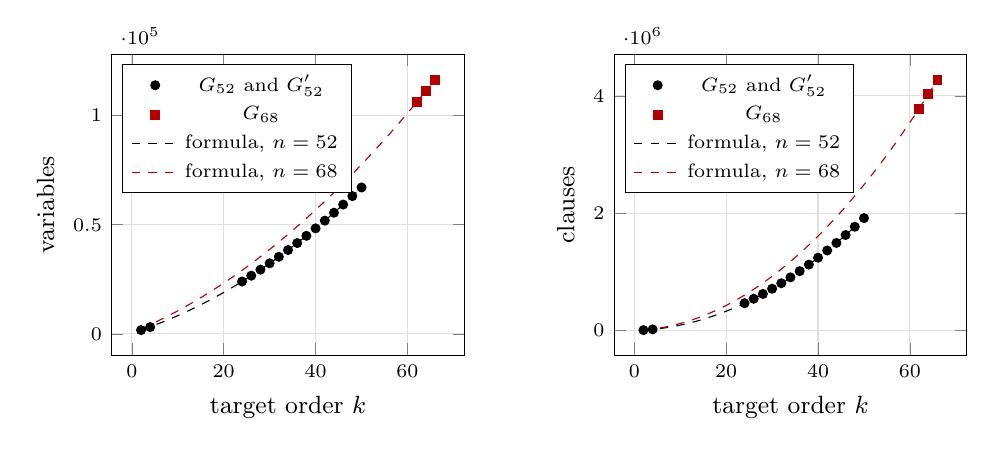
\begin{tikzpicture}
\pgfplotsset{every axis/.append style={tick label style={font=\scriptsize}, label style={font=\small}, legend style={font=\scriptsize}, grid=major, grid style={gray!25}}}
\begin{groupplot}[group style={group size=2 by 1, horizontal sep=1.9cm}, width=0.5\textwidth, height=5.4cm, xlabel={target order $k$}]
\nextgroupplot[ylabel={variables}, legend pos=north west]
\addplot[only marks, mark=*, mark options={solid}, mark size=1.6pt, black] coordinates {(2,1724) (4,3111) (24,23997) (26,26664) (28,29439) (30,32322) (32,35313) (34,38412) (36,41619) (38,44934) (40,48357) (42,51888) (44,55527) (46,59274) (48,63129) (50,67092)};
\addlegendentry{$G_{52}$ and $G'_{52}$}
\addplot[only marks, mark=square*, mark options={solid}, mark size=1.6pt, red!70!black] coordinates {(62,106162) (64,111297) (66,116540)};
\addlegendentry{$G_{68}$}
\addplot[domain=2:50, samples=40, thin, black, dashed] {13*52*x + 8*52 + (27*x^2 - 35*x)/2 + 1};
\addlegendentry{formula, $n=52$}
\addplot[domain=2:66, samples=40, thin, red!70!black, dashed] {13*68*x + 8*68 + (27*x^2 - 35*x)/2 + 1};
\addlegendentry{formula, $n=68$}
\nextgroupplot[ylabel={clauses}, legend pos=north west]
\addplot[only marks, mark=*, mark options={solid}, mark size=1.6pt, black] coordinates {(2,7615) (4,20045) (24,465609) (26,542231) (28,624686) (30,712972) (32,807090) (34,907040) (36,1.01282e+06) (38,1.12444e+06) (40,1.24188e+06) (42,1.36516e+06) (44,1.49427e+06) (46,1.62921e+06) (48,1.76999e+06) (50,1.91659e+06)};
\addlegendentry{$G_{52}$ and $G'_{52}$}
\addplot[only marks, mark=square*, mark options={solid}, mark size=1.6pt, red!70!black] coordinates {(62,3.78553e+06) (64,4.02856e+06) (66,4.27915e+06)};
\addlegendentry{$G_{68}$}
\addplot[domain=2:50, samples=40, thin, black, dashed] {(27*52*x^2 + 73*52*x)/2 + 20*52 + 27*x^2 - 37*x + 1};
\addlegendentry{formula, $n=52$}
\addplot[domain=2:66, samples=40, thin, red!70!black, dashed] {(27*68*x^2 + 73*68*x)/2 + 20*68 + 27*x^2 - 37*x + 1};
\addlegendentry{formula, $n=68$}
\end{groupplot}
\end{tikzpicture}
\caption{Size of the certified formula against the target order $k$, read from the result files (markers) and from the closed forms of Table~\ref{tab:counts} (dashed lines). Left: variables. Right: clauses. The two 52-vertex graphs have the same formula size, so one series stands for both.}\label{fig:size}
\end{figure}


\begin{figure}[tbp]\centering
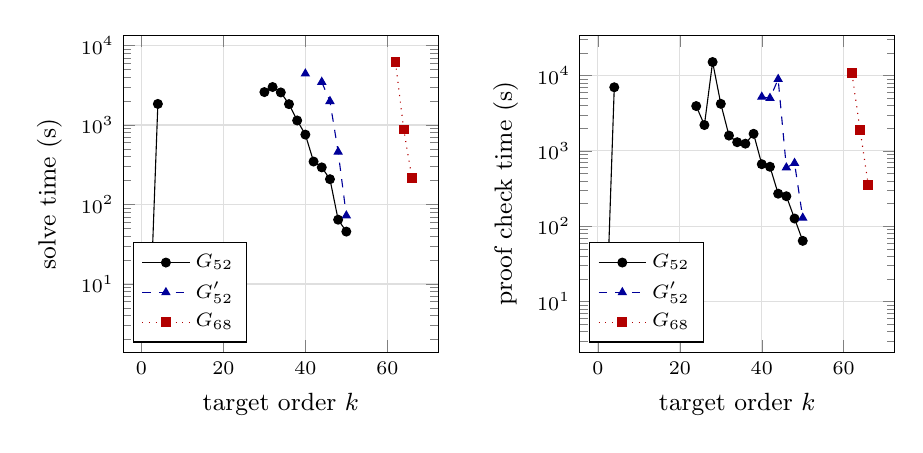
\begin{tikzpicture}
\pgfplotsset{every axis/.append style={tick label style={font=\scriptsize}, label style={font=\small}, legend style={font=\scriptsize}, grid=major, grid style={gray!25}}}
\begin{groupplot}[group style={group size=2 by 1, horizontal sep=1.8cm}, width=0.46\textwidth, height=5.6cm, xlabel={target order $k$}, ymode=log]
\nextgroupplot[ylabel={solve time (s)}, legend pos=south west]
\addplot[mark=*, mark options={solid}, mark size=1.6pt, thin, black, solid] coordinates {(2,2.991) (4,1843.25)};
\addlegendentry{$\Ga$}
\addplot[mark=*, mark options={solid}, mark size=1.6pt, thin, black, solid, forget plot] coordinates {(30,2596.93) (32,3006.86) (34,2570.38) (36,1830.63) (38,1140.52) (40,757.765) (42,347.346) (44,293.321) (46,208.287) (48,64.429) (50,45.654)};
\addplot[mark=triangle*, mark options={solid}, mark size=1.6pt, thin, blue!60!black, dashed] coordinates {(40,4421)};
\addlegendentry{$\Gb$}
\addplot[mark=triangle*, mark options={solid}, mark size=1.6pt, thin, blue!60!black, dashed, forget plot] coordinates {(44,3476.29) (46,1991.15) (48,459.835) (50,72.538)};
\addplot[mark=square*, mark options={solid}, mark size=1.6pt, thin, red!70!black, dotted] coordinates {(62,6203.39) (64,878.069) (66,217.617)};
\addlegendentry{$\Gsix$}
\nextgroupplot[ylabel={proof check time (s)}, legend pos=south west]
\addplot[mark=*, mark options={solid}, mark size=1.6pt, thin, black, solid] coordinates {(2,4.787) (4,6979.24)};
\addlegendentry{$\Ga$}
\addplot[mark=*, mark options={solid}, mark size=1.6pt, thin, black, solid, forget plot] coordinates {(24,3929.3) (26,2200.9) (28,15095.5) (30,4210.22) (32,1595.14) (34,1302.24) (36,1245.61) (38,1684.96) (40,665.239) (42,615.323) (44,270.227) (46,250.022) (48,126.511) (50,63.961)};
\addplot[mark=triangle*, mark options={solid}, mark size=1.6pt, thin, blue!60!black, dashed] coordinates {(40,5196) (42,5002.2) (44,8929.68) (46,599.345) (48,687.347) (50,129.067)};
\addlegendentry{$\Gb$}
\addplot[mark=square*, mark options={solid}, mark size=1.6pt, thin, red!70!black, dotted] coordinates {(62,10654.6) (64,1892.85) (66,348.688)};
\addlegendentry{$\Gsix$}
\end{groupplot}
\end{tikzpicture}
\caption{Wall-clock time of the external solver (left) and of the proof check (right) against the target order $k$, one run per instance, on a logarithmic scale. Instances whose solve time was not recorded are absent from the left panel.}\label{fig:times}
\end{figure}


\begin{figure}[tbp]\centering
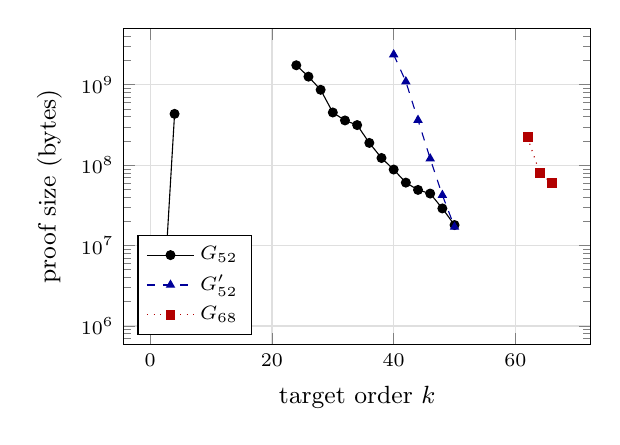
\begin{tikzpicture}
\pgfplotsset{every axis/.append style={tick label style={font=\scriptsize}, label style={font=\small}, legend style={font=\scriptsize}, grid=major, grid style={gray!25}}}
\begin{axis}[width=0.62\textwidth, height=5.6cm, xlabel={target order $k$}, ylabel={proof size (bytes)}, ymode=log, legend pos=south west]
\addplot[mark=*, mark options={solid}, mark size=1.6pt, thin, black, solid] coordinates {(2,1.24721e+06) (4,4.34205e+08)};
\addlegendentry{$\Ga$}
\addplot[mark=*, mark options={solid}, mark size=1.6pt, thin, black, solid, forget plot] coordinates {(24,1.74635e+09) (26,1.26035e+09) (28,8.65404e+08) (30,4.51749e+08) (32,3.59772e+08) (34,3.15072e+08) (36,1.89001e+08) (38,1.22739e+08) (40,8.8201e+07) (42,6.06246e+07) (44,4.92065e+07) (46,4.43313e+07) (48,2.89532e+07) (50,1.79993e+07)};
\addplot[mark=triangle*, mark options={solid}, mark size=1.6pt, thin, blue!60!black, dashed] coordinates {(40,2.37144e+09) (42,1.09408e+09) (44,3.63214e+08) (46,1.20499e+08) (48,4.23903e+07) (50,1.70375e+07)};
\addlegendentry{$\Gb$}
\addplot[mark=square*, mark options={solid}, mark size=1.6pt, thin, red!70!black, dotted] coordinates {(62,2.2093e+08) (64,8.0324e+07) (66,5.96356e+07)};
\addlegendentry{$\Gsix$}
\end{axis}
\end{tikzpicture}
\caption{Size of the DRAT proof of the final formula against the target order $k$, for every refuted order of Table~\ref{tab:orders}. The proofs reach 2.4 GB for the second 52-vertex graph at $k=40$.}\label{fig:proof}
\end{figure}


\paragraph{The controls.} Table~\ref{tab:controls} and Figure~\ref{fig:controls} give the 21 control instances. The formulas with and without the fiber constraints agree in every instance. The Petersen graph is colored by no bridgeless cubic graph of smaller order; $J_5$ is colored by graphs of orders 10 and 12 and of no other order
below 20; $J_3$ is colored by one of order 10 and by none of order 2, 4, 6 or 8; $K_4$ is colored at $k = 2$ and the prism at $k = 2$ and 4, both being 3-edge-colorable. All six satisfiable controls were accepted by the checker and the pipeline's test of their decoded targets found each of them Petersen colorable; all 15 unsatisfiable ones carry a verified proof. All six satisfiable controls returned a vertex map of kind (O): fibers of sizes 1 and 3 for $K_4$ at $k = 2$, 1 and 5 for the prism at $k = 2$,
one fiber of size three and nine singletons for $J_3$ at $k = 10$; no reduced run of a control returned an even kind (the unreduced run of the prism at $k = 2$ returned fibers of sizes 2 and 4), so the even kinds of the formula with the constraints are exercised only through the agreement of the two encodings on the unsatisfiable instances.

\begin{table}[tbp]\centering\footnotesize
\begin{tabular}{llllrrrrrr}
\toprule
 & & & & \multicolumn{3}{c}{with fiber constraints} & \multicolumn{3}{c}{without} \\
\cmidrule(lr){5-7}\cmidrule(lr){8-10}
graph (order) & $k$ & answer & certificate & rounds & cuts & s & rounds & cuts & s\\
\midrule
$K_4$ (4) & 2 & colored & checker accepted & 1 & 0 & 2.7 & 1 & 0 & 2.4 \\
\midrule
prism (6) & 2 & colored & checker accepted & 1 & 0 & 2.4 & 1 & 0 & 2.4 \\
prism (6) & 4 & colored & checker accepted & 1 & 0 & 2.4 & 1 & 0 & 2.7 \\
\midrule
Petersen (10) & 2 & not colored & DRAT verified & 1 & 0 & 4.9 & 1 & 0 & 4.8 \\
Petersen (10) & 4 & not colored & DRAT verified & 1 & 0 & 5.0 & 1 & 0 & 4.9 \\
Petersen (10) & 6 & not colored & DRAT verified & 1 & 0 & 4.9 & 82 & 81 & 5.6 \\
Petersen (10) & 8 & not colored & DRAT verified & 1 & 0 & 4.6 & 139 & 138 & 6.0 \\
\midrule
$J_3$ (12) & 2 & not colored & DRAT verified & 1 & 0 & 4.8 & 1 & 0 & 5.0 \\
$J_3$ (12) & 4 & not colored & DRAT verified & 1 & 0 & 4.5 & 1 & 0 & 5.1 \\
$J_3$ (12) & 6 & not colored & DRAT verified & 1 & 0 & 4.9 & 82 & 81 & 7.7 \\
$J_3$ (12) & 8 & not colored & DRAT verified & 1 & 0 & 5.1 & 184 & 183 & 10.4 \\
$J_3$ (12) & 10 & colored & checker accepted & 1 & 0 & 2.3 & 221 & 220 & 4.2 \\
\midrule
$J_5$ (20) & 2 & not colored & DRAT verified & 1 & 0 & 7.1 & 1 & 0 & 6.6 \\
$J_5$ (20) & 4 & not colored & DRAT verified & 1 & 0 & 44.6 & 1 & 0 & 54.4 \\
$J_5$ (20) & 6 & not colored & DRAT verified & 1 & 0 & 47.4 & 82 & 81 & 77.2 \\
$J_5$ (20) & 8 & not colored & DRAT verified & 1 & 0 & 42.4 & 209 & 208 & 109.6 \\
$J_5$ (20) & 10 & colored & checker accepted & 1 & 0 & 4.7 & 69 & 68 & 3.7 \\
$J_5$ (20) & 12 & colored & checker accepted & 1 & 0 & 2.0 & 36 & 35 & 5.9 \\
$J_5$ (20) & 14 & not colored & DRAT verified & 1 & 0 & 13.6 & 721 & 720 & 153.5 \\
$J_5$ (20) & 16 & not colored & DRAT verified & 1 & 0 & 9.2 & 899 & 898 & 170.6 \\
$J_5$ (20) & 18 & not colored & DRAT verified & 1 & 0 & 8.4 & 1082 & 1081 & 176.6 \\
\bottomrule
\end{tabular}
\caption{The 21 control instances: every even target order $k$ below the order of the graph, for the complete graph on four vertices, the prism, the Petersen graph and the flower snarks $J_3$ and $J_5$. Both encodings give the same answer in every instance. A coloring is accepted by the checker that reads only the graph and the decoded pair and its target is itself Petersen colorable; a refusal carries a DRAT proof accepted by \texttt{drat-trim}. Rounds are solver calls, cuts are lazily learned connectivity and bridge clauses, s is wall-clock seconds.}\label{tab:controls}
\end{table}


\begin{figure}[tbp]\centering
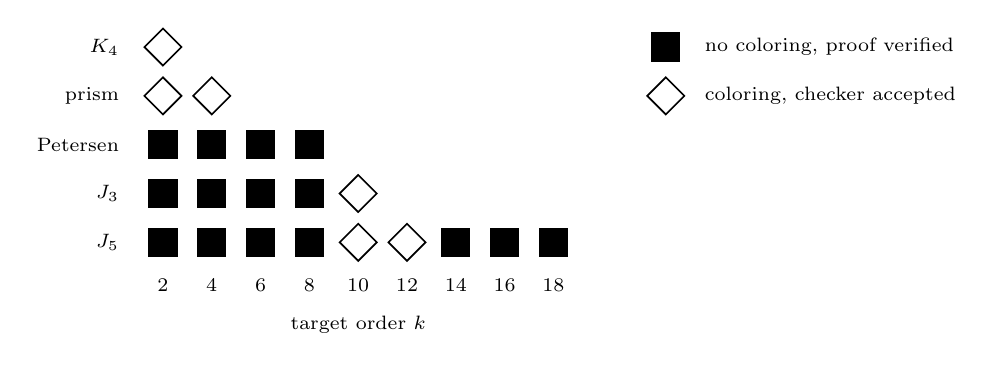
\begin{tikzpicture}[solid, x=0.62cm, y=0.62cm, font=\scriptsize]
\node[anchor=east] at (0.3,0) {$K_4$};
\path[draw, line width=0.6pt] (1.0,0.38) -- (1.38,0) -- (1.0,-0.38) -- (0.62,0) -- cycle;
\node[anchor=east] at (0.3,-1) {prism};
\path[draw, line width=0.6pt] (1.0,-0.62) -- (1.38,-1) -- (1.0,-1.38) -- (0.62,-1) -- cycle;
\path[draw, line width=0.6pt] (2.0,-0.62) -- (2.38,-1) -- (2.0,-1.38) -- (1.62,-1) -- cycle;
\node[anchor=east] at (0.3,-2) {Petersen};
\path[fill=black] (0.7,-2.3) rectangle (1.3,-1.7);
\path[fill=black] (1.7,-2.3) rectangle (2.3,-1.7);
\path[fill=black] (2.7,-2.3) rectangle (3.3,-1.7);
\path[fill=black] (3.7,-2.3) rectangle (4.3,-1.7);
\node[anchor=east] at (0.3,-3) {$J_3$};
\path[fill=black] (0.7,-3.3) rectangle (1.3,-2.7);
\path[fill=black] (1.7,-3.3) rectangle (2.3,-2.7);
\path[fill=black] (2.7,-3.3) rectangle (3.3,-2.7);
\path[fill=black] (3.7,-3.3) rectangle (4.3,-2.7);
\path[draw, line width=0.6pt] (5.0,-2.62) -- (5.38,-3) -- (5.0,-3.38) -- (4.62,-3) -- cycle;
\node[anchor=east] at (0.3,-4) {$J_5$};
\path[fill=black] (0.7,-4.3) rectangle (1.3,-3.7);
\path[fill=black] (1.7,-4.3) rectangle (2.3,-3.7);
\path[fill=black] (2.7,-4.3) rectangle (3.3,-3.7);
\path[fill=black] (3.7,-4.3) rectangle (4.3,-3.7);
\path[draw, line width=0.6pt] (5.0,-3.62) -- (5.38,-4) -- (5.0,-4.38) -- (4.62,-4) -- cycle;
\path[draw, line width=0.6pt] (6.0,-3.62) -- (6.38,-4) -- (6.0,-4.38) -- (5.62,-4) -- cycle;
\path[fill=black] (6.7,-4.3) rectangle (7.3,-3.7);
\path[fill=black] (7.7,-4.3) rectangle (8.3,-3.7);
\path[fill=black] (8.7,-4.3) rectangle (9.3,-3.7);
\node[anchor=north] at (1.0,-4.55) {2};
\node[anchor=north] at (2.0,-4.55) {4};
\node[anchor=north] at (3.0,-4.55) {6};
\node[anchor=north] at (4.0,-4.55) {8};
\node[anchor=north] at (5.0,-4.55) {10};
\node[anchor=north] at (6.0,-4.55) {12};
\node[anchor=north] at (7.0,-4.55) {14};
\node[anchor=north] at (8.0,-4.55) {16};
\node[anchor=north] at (9.0,-4.55) {18};
\node[anchor=north] at (5,-5.3) {target order $k$};
\path[fill=black] (11,-0.3) rectangle (11.6,0.3);
\node[anchor=west] at (11.9,0) {no coloring, proof verified};
\path[draw, line width=0.6pt] (11.3,-1.38) -- (11.68,-1) -- (11.3,-0.62) -- (10.92,-1) -- cycle;
\node[anchor=west] at (11.9,-1) {coloring, checker accepted};
\end{tikzpicture}
\caption{Answers of the 21 control instances of Table~\ref{tab:controls} by graph and target order. The two encodings agree in every cell. The Petersen graph is colored by no graph of smaller order; the flower snark $J_5$ is colored at orders 10 and 12 only, and $J_3$ at order 10 only.}\label{fig:controls}
\end{figure}


\paragraph{The orders without an answer.} Table~\ref{tab:undecided} and Figure~\ref{fig:map} list the orders for which no refutation exists. For $\Ga$ the orders 6 to 22 reached the six-hour cap without an answer: orders 6, 14, 20 and 22 ended at the cap (order 6 after 25 lazy cuts), and orders 8, 10, 12, 16 and 18 were stopped by hand after the in-process solver call held the interpreter lock past the cap. For $\Gb$ no run exists for an order below 40, although the scope
of the sweep extended to every even order. For $\Gsix$ the orders 54 to 60 reached the cap; the run for order 52 was stopped after 4 hours 13 minutes of a 24-hour limit, with three CaDiCaL configurations at full load and proofs of 7.1, 7.9 and 4.4 GB, and its partial proofs were deleted; the formula of 82{,}107 variables and 2{,}683{,}782 clauses is kept for a rerun. The orders 40 to 50 of $\Gsix$ were not attempted.

\begin{table}[tbp]\centering\small
\begin{tabular}{ll>{\raggedright\arraybackslash}p{5.2cm}>{\raggedright\arraybackslash}p{5.6cm}}
\toprule
graph & $k$ & outcome & record\\
\midrule
$\Ga$ & 6 & no answer at the 6 h cap & 25 lazy cuts learned \\
$\Ga$ & 8 & stopped by hand, past the 6 h cap & solver still running \\
$\Ga$ & 10 & stopped by hand, past the 6 h cap & solver still running \\
$\Ga$ & 12 & stopped by hand, past the 6 h cap & solver still running \\
$\Ga$ & 14 & no answer at the 6 h cap & solver still running \\
$\Ga$ & 16 & stopped by hand, past the 6 h cap & solver still running \\
$\Ga$ & 18 & stopped by hand, past the 6 h cap & solver still running \\
$\Ga$ & 20 & no answer at the 6 h cap & solver still running \\
$\Ga$ & 22 & no answer at the 6 h cap & solver still running \\
\midrule
$\Gb$ & 6 to 38 & not attempted & no run exists for an order below 40 \\
\midrule
$\Gsix$ & 54 & no answer at the 6 h cap & formula built, solver still running \\
$\Gsix$ & 56 & no answer at the 6 h cap & formula built, solver still running \\
$\Gsix$ & 58 & no answer at the 6 h cap & formula built, solver still running \\
$\Gsix$ & 60 & no answer at the 6 h cap & formula built, solver still running \\
$\Gsix$ & 52 & stopped at 4 h 13 min of a 24 h limit & formula of 82{,}107 variables and 2{,}683{,}782 clauses \\
$\Gsix$ & 6 to 50 & not attempted & orders 40 to 50 remain open \\
\bottomrule
\end{tabular}
\caption{Target orders for which no refutation or coloring exists, by graph. The runner stops an instance at 21,600 s; in five instances of \(\Ga\) the in-process solver call held the interpreter lock past that limit and was stopped by hand. The formula of order 52 for \(\Gsix\) is kept for a rerun; the partial proofs of the interrupted run were deleted. The orders 2 and 4 are settled for all three graphs by Proposition~\ref{prop:small} and are not listed.}\label{tab:undecided}
\end{table}


\begin{figure}[tbp]\centering
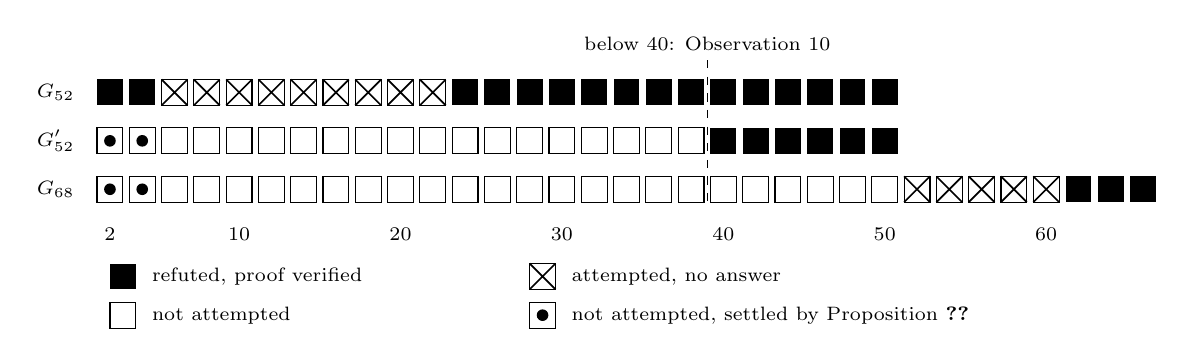
\begin{tikzpicture}[solid, x=0.41cm, y=0.41cm, font=\scriptsize]
\node[anchor=east] at (0.2,0.0) {$\Ga$};
\path[fill=black] (0.6,-0.4) rectangle (1.4,0.4);
\path[fill=black] (1.6,-0.4) rectangle (2.4,0.4);
\path[draw, line width=0.4pt] (2.6,-0.4) rectangle (3.4,0.4);
\draw[line width=0.6pt] (2.6,-0.4) -- (3.4,0.4) (2.6,0.4) -- (3.4,-0.4);
\path[draw, line width=0.4pt] (3.6,-0.4) rectangle (4.4,0.4);
\draw[line width=0.6pt] (3.6,-0.4) -- (4.4,0.4) (3.6,0.4) -- (4.4,-0.4);
\path[draw, line width=0.4pt] (4.6,-0.4) rectangle (5.4,0.4);
\draw[line width=0.6pt] (4.6,-0.4) -- (5.4,0.4) (4.6,0.4) -- (5.4,-0.4);
\path[draw, line width=0.4pt] (5.6,-0.4) rectangle (6.4,0.4);
\draw[line width=0.6pt] (5.6,-0.4) -- (6.4,0.4) (5.6,0.4) -- (6.4,-0.4);
\path[draw, line width=0.4pt] (6.6,-0.4) rectangle (7.4,0.4);
\draw[line width=0.6pt] (6.6,-0.4) -- (7.4,0.4) (6.6,0.4) -- (7.4,-0.4);
\path[draw, line width=0.4pt] (7.6,-0.4) rectangle (8.4,0.4);
\draw[line width=0.6pt] (7.6,-0.4) -- (8.4,0.4) (7.6,0.4) -- (8.4,-0.4);
\path[draw, line width=0.4pt] (8.6,-0.4) rectangle (9.4,0.4);
\draw[line width=0.6pt] (8.6,-0.4) -- (9.4,0.4) (8.6,0.4) -- (9.4,-0.4);
\path[draw, line width=0.4pt] (9.6,-0.4) rectangle (10.4,0.4);
\draw[line width=0.6pt] (9.6,-0.4) -- (10.4,0.4) (9.6,0.4) -- (10.4,-0.4);
\path[draw, line width=0.4pt] (10.6,-0.4) rectangle (11.4,0.4);
\draw[line width=0.6pt] (10.6,-0.4) -- (11.4,0.4) (10.6,0.4) -- (11.4,-0.4);
\path[fill=black] (11.6,-0.4) rectangle (12.4,0.4);
\path[fill=black] (12.6,-0.4) rectangle (13.4,0.4);
\path[fill=black] (13.6,-0.4) rectangle (14.4,0.4);
\path[fill=black] (14.6,-0.4) rectangle (15.4,0.4);
\path[fill=black] (15.6,-0.4) rectangle (16.4,0.4);
\path[fill=black] (16.6,-0.4) rectangle (17.4,0.4);
\path[fill=black] (17.6,-0.4) rectangle (18.4,0.4);
\path[fill=black] (18.6,-0.4) rectangle (19.4,0.4);
\path[fill=black] (19.6,-0.4) rectangle (20.4,0.4);
\path[fill=black] (20.6,-0.4) rectangle (21.4,0.4);
\path[fill=black] (21.6,-0.4) rectangle (22.4,0.4);
\path[fill=black] (22.6,-0.4) rectangle (23.4,0.4);
\path[fill=black] (23.6,-0.4) rectangle (24.4,0.4);
\path[fill=black] (24.6,-0.4) rectangle (25.4,0.4);
\node[anchor=east] at (0.2,-1.5) {$\Gb$};
\path[draw, line width=0.4pt] (0.6,-1.9) rectangle (1.4,-1.1);
\fill (1.0,-1.5) circle (0.18);
\path[draw, line width=0.4pt] (1.6,-1.9) rectangle (2.4,-1.1);
\fill (2.0,-1.5) circle (0.18);
\path[draw, line width=0.4pt] (2.6,-1.9) rectangle (3.4,-1.1);
\path[draw, line width=0.4pt] (3.6,-1.9) rectangle (4.4,-1.1);
\path[draw, line width=0.4pt] (4.6,-1.9) rectangle (5.4,-1.1);
\path[draw, line width=0.4pt] (5.6,-1.9) rectangle (6.4,-1.1);
\path[draw, line width=0.4pt] (6.6,-1.9) rectangle (7.4,-1.1);
\path[draw, line width=0.4pt] (7.6,-1.9) rectangle (8.4,-1.1);
\path[draw, line width=0.4pt] (8.6,-1.9) rectangle (9.4,-1.1);
\path[draw, line width=0.4pt] (9.6,-1.9) rectangle (10.4,-1.1);
\path[draw, line width=0.4pt] (10.6,-1.9) rectangle (11.4,-1.1);
\path[draw, line width=0.4pt] (11.6,-1.9) rectangle (12.4,-1.1);
\path[draw, line width=0.4pt] (12.6,-1.9) rectangle (13.4,-1.1);
\path[draw, line width=0.4pt] (13.6,-1.9) rectangle (14.4,-1.1);
\path[draw, line width=0.4pt] (14.6,-1.9) rectangle (15.4,-1.1);
\path[draw, line width=0.4pt] (15.6,-1.9) rectangle (16.4,-1.1);
\path[draw, line width=0.4pt] (16.6,-1.9) rectangle (17.4,-1.1);
\path[draw, line width=0.4pt] (17.6,-1.9) rectangle (18.4,-1.1);
\path[draw, line width=0.4pt] (18.6,-1.9) rectangle (19.4,-1.1);
\path[fill=black] (19.6,-1.9) rectangle (20.4,-1.1);
\path[fill=black] (20.6,-1.9) rectangle (21.4,-1.1);
\path[fill=black] (21.6,-1.9) rectangle (22.4,-1.1);
\path[fill=black] (22.6,-1.9) rectangle (23.4,-1.1);
\path[fill=black] (23.6,-1.9) rectangle (24.4,-1.1);
\path[fill=black] (24.6,-1.9) rectangle (25.4,-1.1);
\node[anchor=east] at (0.2,-3.0) {$\Gsix$};
\path[draw, line width=0.4pt] (0.6,-3.4) rectangle (1.4,-2.6);
\fill (1.0,-3.0) circle (0.18);
\path[draw, line width=0.4pt] (1.6,-3.4) rectangle (2.4,-2.6);
\fill (2.0,-3.0) circle (0.18);
\path[draw, line width=0.4pt] (2.6,-3.4) rectangle (3.4,-2.6);
\path[draw, line width=0.4pt] (3.6,-3.4) rectangle (4.4,-2.6);
\path[draw, line width=0.4pt] (4.6,-3.4) rectangle (5.4,-2.6);
\path[draw, line width=0.4pt] (5.6,-3.4) rectangle (6.4,-2.6);
\path[draw, line width=0.4pt] (6.6,-3.4) rectangle (7.4,-2.6);
\path[draw, line width=0.4pt] (7.6,-3.4) rectangle (8.4,-2.6);
\path[draw, line width=0.4pt] (8.6,-3.4) rectangle (9.4,-2.6);
\path[draw, line width=0.4pt] (9.6,-3.4) rectangle (10.4,-2.6);
\path[draw, line width=0.4pt] (10.6,-3.4) rectangle (11.4,-2.6);
\path[draw, line width=0.4pt] (11.6,-3.4) rectangle (12.4,-2.6);
\path[draw, line width=0.4pt] (12.6,-3.4) rectangle (13.4,-2.6);
\path[draw, line width=0.4pt] (13.6,-3.4) rectangle (14.4,-2.6);
\path[draw, line width=0.4pt] (14.6,-3.4) rectangle (15.4,-2.6);
\path[draw, line width=0.4pt] (15.6,-3.4) rectangle (16.4,-2.6);
\path[draw, line width=0.4pt] (16.6,-3.4) rectangle (17.4,-2.6);
\path[draw, line width=0.4pt] (17.6,-3.4) rectangle (18.4,-2.6);
\path[draw, line width=0.4pt] (18.6,-3.4) rectangle (19.4,-2.6);
\path[draw, line width=0.4pt] (19.6,-3.4) rectangle (20.4,-2.6);
\path[draw, line width=0.4pt] (20.6,-3.4) rectangle (21.4,-2.6);
\path[draw, line width=0.4pt] (21.6,-3.4) rectangle (22.4,-2.6);
\path[draw, line width=0.4pt] (22.6,-3.4) rectangle (23.4,-2.6);
\path[draw, line width=0.4pt] (23.6,-3.4) rectangle (24.4,-2.6);
\path[draw, line width=0.4pt] (24.6,-3.4) rectangle (25.4,-2.6);
\path[draw, line width=0.4pt] (25.6,-3.4) rectangle (26.4,-2.6);
\draw[line width=0.6pt] (25.6,-3.4) -- (26.4,-2.6) (25.6,-2.6) -- (26.4,-3.4);
\path[draw, line width=0.4pt] (26.6,-3.4) rectangle (27.4,-2.6);
\draw[line width=0.6pt] (26.6,-3.4) -- (27.4,-2.6) (26.6,-2.6) -- (27.4,-3.4);
\path[draw, line width=0.4pt] (27.6,-3.4) rectangle (28.4,-2.6);
\draw[line width=0.6pt] (27.6,-3.4) -- (28.4,-2.6) (27.6,-2.6) -- (28.4,-3.4);
\path[draw, line width=0.4pt] (28.6,-3.4) rectangle (29.4,-2.6);
\draw[line width=0.6pt] (28.6,-3.4) -- (29.4,-2.6) (28.6,-2.6) -- (29.4,-3.4);
\path[draw, line width=0.4pt] (29.6,-3.4) rectangle (30.4,-2.6);
\draw[line width=0.6pt] (29.6,-3.4) -- (30.4,-2.6) (29.6,-2.6) -- (30.4,-3.4);
\path[fill=black] (30.6,-3.4) rectangle (31.4,-2.6);
\path[fill=black] (31.6,-3.4) rectangle (32.4,-2.6);
\path[fill=black] (32.6,-3.4) rectangle (33.4,-2.6);
\node[anchor=north] at (1.0,-3.9) {2};
\node[anchor=north] at (5.0,-3.9) {10};
\node[anchor=north] at (10.0,-3.9) {20};
\node[anchor=north] at (15.0,-3.9) {30};
\node[anchor=north] at (20.0,-3.9) {40};
\node[anchor=north] at (25.0,-3.9) {50};
\node[anchor=north] at (30.0,-3.9) {60};
\draw[dashed, line width=0.5pt] (19.5,1) -- (19.5,-3.5);
\node[anchor=south] at (19.5,1) {below 40: Observation~10};
\path[fill=black] (1,-6.1) rectangle (1.8,-5.3);
\node[anchor=west] at (2,-5.699999999999999) {refuted, proof verified};
\path[draw, line width=0.4pt] (14,-6.1) rectangle (14.8,-5.3);
\draw[line width=0.6pt] (14,-6.1) -- (14.8,-5.3) (14,-5.3) -- (14.8,-6.1);
\node[anchor=west] at (15,-5.699999999999999) {attempted, no answer};
\path[draw, line width=0.4pt] (1,-7.3) rectangle (1.8,-6.5);
\node[anchor=west] at (2,-6.8999999999999995) {not attempted};
\path[draw, line width=0.4pt] (14,-7.3) rectangle (14.8,-6.5);
\fill (14.4,-6.8999999999999995) circle (0.18);
\node[anchor=west] at (15,-6.8999999999999995) {not attempted, settled by Proposition~\ref{prop:small}};
\end{tikzpicture}
\caption{Status of every even target order $k$ below the order of the graph, one cell per order from 2 (left) to $n-2$, for the three graphs of the sweep. The dashed line marks the bound of the cited observation, below which a smaller counterexample is excluded without computation. The cell $k=52$ of the 68-vertex graph is a run stopped before any answer.}\label{fig:map}
\end{figure}


\paragraph{What the theorems say about the undecided orders.} The refuted orders suffice for Theorem~\ref{thm:h3}, because the cited observation excludes the orders below 40. For the unconditional statement that no connected bridgeless cubic graph of order below 52 colors $\Ga$ the orders 6 to 22 of $\Ga$ and 6 to 38 of $\Gb$ would
have to be decided, since 2 and 4 are settled by Proposition~\ref{prop:small}. Those orders are smaller than the smallest ones decided for these graphs, and the cost of the decided orders grows as the order falls (Figure~\ref{fig:times}).

\section{Ablation: what the fiber constraints contribute}\label{sec:ablation}

The fiber constraints are the only component of the method that changes what a solver can decide, so the ablation removes them: the baseline is the formula without the parity chains, the unit clause on the last-but-one target and the forced $q$, which is the formula of the first attempt. Two measurements compare the baseline with the full formula.

On the target graph, the first attempt ran the ten orders from $k = 32$ to $k = 50$ of $\Ga$ at once with the baseline. After about 35 minutes each of the ten orders had learned between 1{,}800 and 2{,}400 lazy cuts, more than 95 percent of them bridge cuts, at roughly one cut per second and with no sign of convergence; no order was decided and the attempt was stopped (Table~\ref{tab:ablation-orders}).
The explanation is the free part of the target: the unused target vertices form a part of $H$ that $G$ does not constrain, and the solver enumerates its bridged completions one by one. With the fiber constraints each of the same ten orders was refuted with no lazy cut at all, in 137 s ($k = 50$) to 5{,}882 s ($k = 32$) of wall-clock time per run, solve and check included. The figures of the first attempt are the ones recorded
when it was stopped; its log files are not in the repository, and the comparison is therefore between recorded totals and not between two runs under the same load.

\begin{table}[tbp]\centering\small
\begin{tabular}{>{\raggedright\arraybackslash}p{3.0cm}>{\raggedright\arraybackslash}p{2.4cm}>{\raggedright\arraybackslash}p{3.4cm}>{\raggedright\arraybackslash}p{1.6cm}>{\raggedright\arraybackslash}p{2.8cm}}
\toprule
formula & orders run & lazy cuts per order & orders decided & wall clock\\
\midrule
without the fiber constraints & 10 ($32 \le k \le 50$) & 1,800 to 2,400, over 95 percent bridge cuts & 0 & stopped after about 35 min \\
with the fiber constraints & 10 ($32 \le k \le 50$) & 0 & 10 & 137 to 5{,}882 s per order \\
\bottomrule
\end{tabular}
\caption{Effect of the fiber constraints on the first graph at the ten target orders from 32 to 50. The figures for the formula without the constraints are those recorded when that attempt was stopped; the figures for the formula with them are the wall-clock seconds of the ten decided runs (solve and proof check included).}\label{tab:ablation-orders}
\end{table}

\begin{table}[tbp]\centering\small
\begin{tabular}{lrrrrrr}
\toprule
 & & \multicolumn{2}{c}{with fiber constraints} & \multicolumn{3}{c}{without} \\
\cmidrule(lr){3-4}\cmidrule(lr){5-7}
graph & instances & cuts & s & instances with a cut & cuts & s\\
\midrule
$K_4$ & 1 & 0 & 3 & 0 & 0 & 2 \\
prism & 2 & 0 & 5 & 0 & 0 & 5 \\
Petersen & 4 & 0 & 19 & 2 & 219 & 21 \\
$J_3$ & 5 & 0 & 22 & 3 & 484 & 32 \\
$J_5$ & 9 & 0 & 179 & 7 & 3{,}091 & 758 \\
\midrule
all & 21 & 0 & 228 & 12 & 3{,}794 & 819 \\
\bottomrule
\end{tabular}
\caption{Effect of the fiber constraints on the 21 control instances of Table~\ref{tab:controls}, summed by graph: lazily learned cuts and wall-clock seconds with and without the constraints, and the number of instances in which the formula without them needed at least one cut.}\label{tab:ablation-controls}
\end{table}


On the 21 controls the same effect can be measured run by run, under the same runner (Table~\ref{tab:ablation-controls} and Figure~\ref{fig:ablation}). With the fiber constraints no control needed a lazy cut and the 21 runs took 228 s in all. Without them 12 of the 21 instances needed at least one cut, 3{,}794 cuts were learned in total, and the runs took 819 s; the instances at the largest orders are the ones that
suffer: $J_5$ at $k = 18$ learned 1{,}081 cuts in 176.6 s against none in 8.4 s, a factor of 21. The cuts grow with the order of the target (for $J_5$: 720, 898 and 1{,}081 at $k = 14$, 16 and 18), which is the behavior that stopped the first attempt at the orders of $\Ga$ and $\Gb$. The ablation is small in two respects: it is one run per cell, and its target instances are the controls and one graph at one family of orders,
so it supports the claim that the constraints are necessary for the sweep at its scale, not an estimate of the speed-up as a function of the order.

\begin{figure}[tbp]\centering
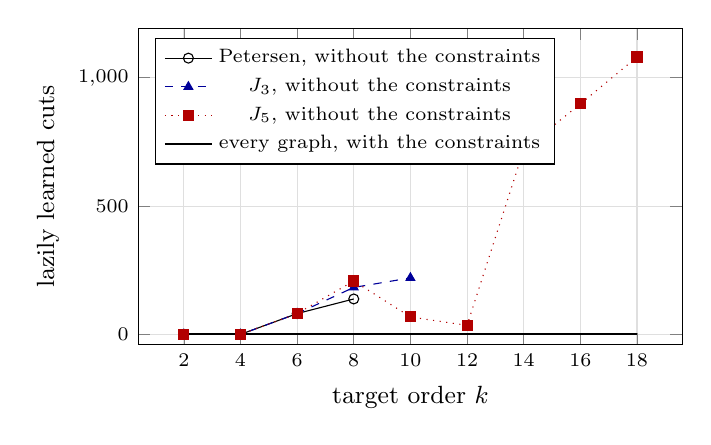
\begin{tikzpicture}
\pgfplotsset{every axis/.append style={tick label style={font=\scriptsize}, label style={font=\small}, legend style={font=\scriptsize}, grid=major, grid style={gray!25}}}
\begin{axis}[width=0.7\textwidth, height=5.6cm, xlabel={target order $k$}, ylabel={lazily learned cuts}, legend pos=north west, ymin=-40, xtick={2,4,6,8,10,12,14,16,18}]
\addplot[mark=o, mark options={solid}, mark size=1.8pt, thin, black, solid] coordinates {(2,0) (4,0) (6,81) (8,138)};
\addlegendentry{Petersen, without the constraints}
\addplot[mark=triangle*, mark options={solid}, mark size=1.8pt, thin, blue!60!black, dashed] coordinates {(2,0) (4,0) (6,81) (8,183) (10,220)};
\addlegendentry{$J_3$, without the constraints}
\addplot[mark=square*, mark options={solid}, mark size=1.8pt, thin, red!70!black, dotted] coordinates {(2,0) (4,0) (6,81) (8,208) (10,68) (12,35) (14,720) (16,898) (18,1081)};
\addlegendentry{$J_5$, without the constraints}
\addplot[thick, black, domain=2:18] {0};
\addlegendentry{every graph, with the constraints}
\end{axis}
\end{tikzpicture}
\caption{Lazily learned connectivity and bridge cuts on the control instances against the target order $k$: the formula without the fiber constraints (markers) and the formula with them (solid line at zero, all 21 instances). The number of cuts of the formula without the constraints grows with the order.}\label{fig:ablation}
\end{figure}


The other components of the method are not ablated. The symmetry breaking was not run without, on the target graphs; its effect is known only on the Petersen-colorability formula of three graphs, where removing the symmetry breaking multiplied the solving time by factors from about 4 to 15 and the checking time by factors from about 7 to 22 (for $\Ga$, 1.8 s against 27.6 s of solving and 1.2 s against 26.5 s of checking)
in the earlier certification runs of the programme. The attach clauses cannot change a result: they are implied by the base formula (Proposition~\ref{prop:attach}).

\section{Discussion}\label{sec:discussion}

\paragraph{What the results establish.} For both 52-vertex counterexamples every even target order from 40 to 50 is refuted with a verified proof; for the first one so are the orders 2, 4 and 24 to 38. Combined with the exhaustive computation of~\cite{GJMMMU2026}, which excludes every smaller order, the two graphs are colorable only by themselves
(Theorem~\ref{thm:h3}); the part that is established here, Theorem~\ref{thm:orders}, does not depend on that computation. The result answers the question of~\cite[Section~5.4]{GJMMMU2026} for both graphs, conditionally. It also gives the three
kinds of colorings that any smaller bridgeless cubic graph would have to realize, and the formulas that decide each order.

\paragraph{Smallest counterexamples.} A smallest counterexample to the Petersen coloring conjecture belongs to $\Hthree$, and its order lies between 40 and 52~\cite{GJMMMU2026}. Membership of $\Ga$ and $\Gb$ in $\Hthree$ is necessary for them to be smallest counterexamples; it is not sufficient, since $\Hthree$ may contain graphs of different orders that do not color
one another. The results are consistent with the 52-vertex graphs being smallest, and do not decide it: a smaller counterexample, if any, would have an order between 40 and 50 and need not color either 52-vertex graph.

\paragraph{The other known counterexamples.} The same question is open for the counterexample on 68 vertices, for which the target orders 62, 64 and 66 are refuted, the order 52 was stopped before an answer, the orders 54 to 60 reached the cap and the orders 40 to 50 were not attempted (Table~\ref{tab:undecided}), and for the two on 112 vertices, for which no run exists. An affirmative answer to ``is it colored by a smaller bridgeless cubic graph'' for the
68-vertex graph would exhibit a smaller counterexample, possibly one of $\Ga$, $\Gb$, and the order 52 is the most informative first target. The formulas of Section~\ref{sec:method} apply without change; the largest has target order 110.

\paragraph{Why the fiber lemmas matter.} Without Lemmas~\ref{lem:parity} and~\ref{lem:unused} the unknown target has vertices and edges that no edge of $G$ constrains. For $\Ga$ the loop of Section~\ref{sec:pipeline} then produced, for each of the ten target orders from 32 to 50, between 1{,}800 and 2{,}400 targets with a bridge in half an hour, each excluded by one clause, without deciding any order. With the lemmas every edge of
the target is the image of an edge of $G$, and every order was decided without a single such clause. The lemmas do not make the problem easy: the cost still grows steeply as the order falls and the second graph costs more than the first at equal order.

\paragraph{Scope of the small orders.} Proposition~\ref{prop:small} shows that the target orders 2 and 4 carry no information for a graph that is not 3-edge-colorable, and that the rows $k=2,4$ of the first graph are a consistency check of the encoder. The orders that remain open for the unconditional statement are 6 to 22 for $\Ga$ and 6 to 38 for $\Gb$; the nearest decided orders of $\Ga$, $k = 24$ to 30, took between 2{,}597 s (at $k = 30$) and more than the six-hour cap (at $k = 24$ to 28, times not recorded), with proofs between 0.45 and 1.75 GB, and the undecided orders lie below them.

\paragraph{A question.} Is there a counterexample to the Petersen coloring conjecture that is colored by a smaller counterexample? By Lemma~\ref{lem:parity} the fibers of such a coloring are all odd or all even, and by Proposition~\ref{prop:nminus2} a coloring with every target vertex used needs target order at most $n - 4$ when the graph is simple and has no triangles. A satisfiable $F_{G,k}$ for a counterexample $G$ whose decoded target is connected and bridgeless would answer the question affirmatively, since a graph that colors a counterexample is a counterexample.

\section{Limitations}\label{sec:limitations}

\paragraph{External computation.} Theorem~\ref{thm:h3} is conditional on Observation~10 of~\cite{GJMMMU2026}, whose proof for the orders up to 38 is an exhaustive check of the weak snarks on 38 vertices that took about 12 CPU-years. That computation is not reproduced here. The unconditional part of the result is Theorem~\ref{thm:orders}; the membership in $\Hthree$ without the observation needs the undecided orders (Table~\ref{tab:undecided}).

\paragraph{The encoder is trusted code.} The symmetry breaking and the fiber constraints are proved sound on paper (Propositions~\ref{prop:symmetry} and~\ref{prop:fibers}), and the sizes and hashes of all formulas are reproduced by the generator, but the encoder has not been shown to be correct on a satisfiable instance at the scale of the claim. Every positive control has at most 20 vertices and a target of order at most 12, and the only
computations at the scale of the claim (52 or 68 vertices, target orders 40 to 66) end in unsatisfiable answers. A defect of the encoder that over-constrains large instances, for example in the symmetry breaking, would show up only as more unsatisfiable answers. A test with a planted satisfiable case, a graph known to be colored by a graph of 40 to 52 vertices, such as a double cover of $\Ga$ at $k = 52$, together with a corrupted-target
negative control, would close the gap; it is not part of this paper, and no claim here depends on its outcome. The satisfiable reduced controls return only vertex maps of kind (O), so the even kinds are tested only by agreement on unsatisfiable instances.

\paragraph{Certificates and tool versions.} The proofs, up to 2.4 GB each, are kept outside the repository; the repository holds the hashes of the formulas and of the proofs (Appendix~\ref{app:hashes}), the result files, and the generator that rebuilds every formula and its hash. A third party can rebuild each formula and compare its hash, but must run the solver and the checker again, for hours, to obtain a proof. The version of the external
CaDiCaL (1.7.3, from the manifests of the earlier certification runs on the same machine), of \texttt{drat-trim}, of PySAT and the processor model were not recorded with the experiment, so these are not stated with certainty here; the proofs would be identical only under the same solver build and options.

\paragraph{Timings and the shared machine.} Each time in Tables~\ref{tab:orders} and~\ref{tab:ablation-orders} is one wall-clock measurement taken while other computations shared the machine; the experiment has no repetitions, so no standard deviation or confidence interval exists, and the times show orders of magnitude and a trend, not precise costs. The comparison with the first attempt uses recorded totals whose log files are not in the repository.

\paragraph{Incidents of the runs.} Several runs ended outside the design. The watchdog of the runner is a timer thread that cannot fire while the in-process solver holds the interpreter lock, so five runs of $\Ga$ (orders 8, 10, 12, 16, 18) and one of $\Gb$ ran past the cap and were stopped by hand. A driver script of the stopped first attempt kept starting instances with the unreduced code and shared logs with the reduced runs of orders
12 to 30 for four hours before it was found and killed; no result file came from it, because every result carries the reduced flag and its own certificate, and the logs of orders 12 to 30 are not used as evidence. A stop of the virtual machine killed three proof checks, which were redone on complete proofs. These incidents change which orders are undecided and the recorded times; they do not affect the verified proofs.

\paragraph{Scope.} The sweep covers three graphs and even target orders; the two 112-vertex graphs, the cyclically 5-edge-connected counterexamples of~\cite{GJMMMU2026} and the 68-vertex graph below order 62 are not covered. The title carries the condition on which membership in $\Hthree$ rests, Observation~10; the abstract and Theorem~\ref{thm:h3} state the same dependence.

\section{Reproducibility and data availability}\label{sec:reproducibility}

The edge lists, encoders, checkers, runners, results and the hashes of all formulas and proofs are in the repository \url{https://github.com/fsantibanezleal/CAOS_RESEARCH}, under \path{problems/combinatorics/petersen-coloring/}. \raggedright The computation is archived in \path{experiments/EXP-007-colorable-only-by-itself} (EXP below) and the encoder is \path{code/pcclib/hcolor.py}.
The result files are \path{artifacts/result-<graph>-k<k>.json} for the target orders, and the same name with the suffix \path{-red} or \path{-unred} for the controls. The manuscript is in \path{manuscripts/petersen-coloring/colorable-only-by-itself}, called MS below. The commands, run from the repository root, are the following.
\begin{verbatim}
python EXP/run_inc.py --graph G52 --k 50 --cap 21600
python EXP/certify_existing.py --graph G52b --k 42 --timeout 80000
EXP/portfolio_certify.sh <cnf> <proof-prefix> <result-json> \
    <solve-limit-s> <check-limit-s>
python EXP/write_formula.py --graph G68 --k 52
sh EXP/agreement.sh
python MS/make_tables.py
python MS/make_tables.py --check-hashes
python MS/assemble.py
\end{verbatim}
The first command solves one instance with the in-process solver and the external solver and checker; the flag \texttt{-{}-unreduced} selects the baseline formula without the fiber constraints and \texttt{-{}-suffix} names the result file. The second checks a formula and proof pair left on disk after the runner's cap. The third, run inside WSL, is the portfolio on a formula file, and
the fourth writes the formula of an instance (and with \texttt{-{}-decode} decodes a model). The fifth runs the 21 controls. The sixth writes the tables and figures of this paper from the result files and checks the variable and clause counts of Table~\ref{tab:counts} against them. The seventh rebuilds the 25 certified formulas and the kept formula of $\Gsix$ at $k = 52$ with the encoder and compares the SHA-256
of each DIMACS file with the value of Appendix~\ref{app:hashes} (Table~\ref{tab:hashes}); the eighth assembles the source, which is built by three passes of \texttt{pdflatex}. The formulas and proofs are written to the data root of the experiment, outside the repository; the 2.4 GB proof for $\Gb$ at $k = 40$ is the largest.

\section{Conclusions}\label{sec:conclusions}

Two lemmas on the vertex map of an $H$-coloring, the parity of its fibers and the reduction of its unused vertices, turn the question whether a cubic graph is colored by a smaller bridgeless cubic graph into one propositional formula per even target order, with the target graph unknown and no part of it free.
With the formula stated in full, its symmetry breaking proved sound, and every refutation certified by a DRAT proof, both 52-vertex counterexamples to the Petersen coloring conjecture have every even target order from 40 to 50 refuted, and the first one also the orders 2, 4 and 24 to 38. Assuming Observation~10 of~\cite{GJMMMU2026}, both belong to $\Hthree$: they are colorable only by themselves, and
the smallest counterexample question for them is unchanged. The next steps are the undecided orders (6 to 22 of $\Ga$, 6 to 38 of $\Gb$) for an unconditional proof; a planted satisfiable test at the scale of the claim for the encoder; and the 68-vertex graph, starting with the order 52.

\appendix

\section{SHA-256 hashes of the formulas and proofs}\label{app:hashes}

Table~\ref{tab:hashes} gives, for every refuted order, the SHA-256 of the DIMACS file of the certified formula and of its DRAT proof, and the hash of the kept formula of order 52 of $\Gsix$. The formula file is written by the runner with one comment line before the header line, of the form \texttt{c EXP-007 <tag> final formula: base + <a> attach + 0 learned cuts}, where the tag
is the graph and order (for $\Gb$ at $k = 40$ the tag of the portfolio run, \texttt{G52b\_k40-long}) and $a = k - 1$; the comment line is part of the hashed bytes, which is why the hash depends on the tag. Rebuilding the formula with the encoder and writing the same comment reproduces every first value of the table, which is what \texttt{make\_tables.py -{}-check-hashes} checks. The second
value of each pair is the hash of the proof file produced by the solver; it can be compared only with a proof file kept from the original run.

\begin{longtable}{@{}rrll@{}}
\caption{SHA-256 of the certified formula (the DIMACS file, comment line included) and of the DRAT proof, for every refuted target order, and of the formula of order 52 for the 68-vertex graph. Regenerating a formula with the command of Section~\ref{sec:reproducibility} and hashing it reproduces the first value of each pair.}\label{tab:hashes}\\
\toprule
graph & $k$ & object & SHA-256\\
\midrule
\endfirsthead
\toprule
graph & $k$ & object & SHA-256\\
\midrule
\endhead
\bottomrule
\endfoot
\bottomrule
\endlastfoot
$\Ga$ & 50 & formula & {\tiny\ttfamily 58ddbf0f3787268d9446d2b584ec938539af68a63805ed903a04d52a37f241c0} \\
 & & proof & {\tiny\ttfamily 949c1eb1a7652d08a6585c1ca76c4e019fe211d26c41292e3d6c64d0c5c5f7b9} \\
$\Ga$ & 48 & formula & {\tiny\ttfamily 611f6b1167d13d6d436b72041350670f923d3ab47472437340ec9f30680365a4} \\
 & & proof & {\tiny\ttfamily 8acae5c66a40460d09be8b2fd7a9f6ac5abfdc05e490d1f5bfff8b2eac378c34} \\
$\Ga$ & 46 & formula & {\tiny\ttfamily 633f455fae62cf1cabee9b678943ebe7cdec958668e767d78b3f27fb38da838a} \\
 & & proof & {\tiny\ttfamily c79aa9efefaf8054064d2188c8d6ca200c677377b98be5f225d453687e5cd792} \\
$\Ga$ & 44 & formula & {\tiny\ttfamily d3edaa17bd2d59cffabb6ba356fe42986db1400b9bac65b3280754d9dde81b6d} \\
 & & proof & {\tiny\ttfamily dc812433a47e3d3df27aee1cd7bee209d205169f77d6cdab2fd83041874addad} \\
$\Ga$ & 42 & formula & {\tiny\ttfamily d1f1eb1bf27a201fd2821b42f878d8aa03eba2d666f639552e398ea26f2f9dad} \\
 & & proof & {\tiny\ttfamily d7a471402177a5a90e0db18b72d97f523d5b0732ae01ad70d1860f081b74e1c4} \\
$\Ga$ & 40 & formula & {\tiny\ttfamily c7fd45857e995c8892454c785185684723c777af30d9d55449ff8fad87ec9e07} \\
 & & proof & {\tiny\ttfamily 3b8fd3da35ca262558b8c574fb15b6e9b3d61cff2460a7e29ac1e7fd0975e355} \\
$\Ga$ & 38 & formula & {\tiny\ttfamily 483e879321833820303209a422dbeb9d1fc2e66c53087667953c8fdab87f8c60} \\
 & & proof & {\tiny\ttfamily dd4843c7816b9be60ad3612312a189f3adbcffc1b74fd85e6229571c01747d54} \\
$\Ga$ & 36 & formula & {\tiny\ttfamily 8db800ccb7e38c0505ab8e10c0a89174b94dfa177175f1df159f675dcc860f5b} \\
 & & proof & {\tiny\ttfamily 33577bd03c79978a3f585da3d1a25b5f77a6e56a927c9eae0de4281579644d12} \\
$\Ga$ & 34 & formula & {\tiny\ttfamily 25d33f7976acd23311cf89bce185baaa7933a1928e052efe43e84040e1cf3635} \\
 & & proof & {\tiny\ttfamily 933cc75be39059ea8a88c8cb194bc0fa9146075c15c82f7f466d8d5e73157c2b} \\
$\Ga$ & 32 & formula & {\tiny\ttfamily d08f4241728ed252047e603d01982532fd306915be6d2effa633095ec505b07d} \\
 & & proof & {\tiny\ttfamily 8ff33d874ca72250904f8f2bedaa41ba6af0c9989063192650834fd826e805fa} \\
$\Ga$ & 30 & formula & {\tiny\ttfamily 7b8eceb8cee99711d60e7db38293c497baa4b835de043126e1a5df5d4d15a4b9} \\
 & & proof & {\tiny\ttfamily c912caeb207ea1b809fab1b55445fcdf1c726cc60b7a5dc3deba3c225c749946} \\
$\Ga$ & 28 & formula & {\tiny\ttfamily bfd177f3d3dcb336c1df6e6b12c93dcd71dfbf32362b48dfedaecfed0ff73634} \\
 & & proof & {\tiny\ttfamily dc100d4cd25425d9d92f2ce5fff7c03f2ddf17e25ed18233914f23e2a96c579b} \\
$\Ga$ & 26 & formula & {\tiny\ttfamily 92751161f0b984bcaa03a2d54b0f4aa807283637fb4db0f6886637cb5c8b1d14} \\
 & & proof & {\tiny\ttfamily 701090ce92822b7eb100bd704b737b1b5721ad1bb07c6639aa0c95fcf704b626} \\
$\Ga$ & 24 & formula & {\tiny\ttfamily b75a49d39248c7aa3b387c40fe9cfe8fbe4829aea391910ca48a85a1ececacca} \\
 & & proof & {\tiny\ttfamily fbc99c3bf0a7f7b6c0d1c82aff95f293d0ef594b5ed4a802d0c7499c86c0841d} \\
$\Ga$ & 4 & formula & {\tiny\ttfamily f577c10a601a57119573c947060cbbeb868890a9fddf0b292e0ae5372ad90173} \\
 & & proof & {\tiny\ttfamily b74ca055315f05eeac3f18b025963b5a0c83bb48f4cd4a8a147e87f929e01818} \\
$\Ga$ & 2 & formula & {\tiny\ttfamily 8ea582646621cf507685369af6fc2e08ca50521fd9cb8229ad80aaffd4d119f3} \\
 & & proof & {\tiny\ttfamily 813a578137567e65444aab7350806db3399d2e8c4518c0c4079c0f2f653d2305} \\
$\Gb$ & 50 & formula & {\tiny\ttfamily a1427391b8df723678386a67412b511e30965b535cdd5c486564c45ed64ccded} \\
 & & proof & {\tiny\ttfamily 9aaa861134dee114412ca015c27891f087cb1bc07f57d4b17e0cf415e8a91acb} \\
$\Gb$ & 48 & formula & {\tiny\ttfamily 2b787144e96814bb0b5c15a7aa70a72e28fc11da296260bfbc16339677ef21dc} \\
 & & proof & {\tiny\ttfamily 9c3012e166aa952b4c1cdd83778dc89bf92587f0d6bfa227ac757cd0316ec566} \\
$\Gb$ & 46 & formula & {\tiny\ttfamily 34d490e354d2f3fa0441102f5a431d33e90744a22887bc0a4f908f9356a3d3a6} \\
 & & proof & {\tiny\ttfamily db4beab34704e0a0a19648ee72f2ff7082ba85c6c1f4cc997c8114567d6f7641} \\
$\Gb$ & 44 & formula & {\tiny\ttfamily 128ca9c2655e76dc6e9e2a0d8dba82ab8feb8f892541e8e5b09a4ff71bf1efa8} \\
 & & proof & {\tiny\ttfamily c438bbb52ed9ab82b8ef5821f1cc0c8ebb3932e082f05b88d99164b5d3f9153e} \\
$\Gb$ & 42 & formula & {\tiny\ttfamily d27ccfdd1f996bb8fe53758b58a6f275ceee0da36cc57fbb773b565e31aa3808} \\
 & & proof & {\tiny\ttfamily aafd1a0db6908e80dd7b37fc3c315421f86ceedbf0241cc2bf1c687ae7cb333a} \\
$\Gb$ & 40 & formula & {\tiny\ttfamily dfe81aa700c9cb190a3e7d62bc7dc6c5d4c0ed73fcb6d4e0bb65d5dbb4fec62e} \\
 & & proof & {\tiny\ttfamily 7abe12eb57336e4e4eadb594da989c64072e5325b7af8e63590d04472df2ad2b} \\
$\Gsix$ & 66 & formula & {\tiny\ttfamily 295c28183652837ad12345941964a4ce1db2ba28793645eb279c3ce0c3065638} \\
 & & proof & {\tiny\ttfamily 6751fc91c98be224c7f6d513ba2c1da2bcfe771ab2a2274ff0f656a86e6b78a5} \\
$\Gsix$ & 64 & formula & {\tiny\ttfamily fc7c229ee30c1aaa0ffce94c9fa420f732bbfb8da66beb3081357104aa16cd9d} \\
 & & proof & {\tiny\ttfamily e149d052d6046886bc5d4349e1cad4c159600fecc7e9f65a282013d4ffcb4ea2} \\
$\Gsix$ & 62 & formula & {\tiny\ttfamily c454092db64fd753df3d5833e6876fe0eadef4242c8de9663649930eab1d5de0} \\
 & & proof & {\tiny\ttfamily 440c53b31d3b03c50fe1438330c083d2b085deb800dee04244543d52a7fe43ca} \\
$\Gsix$ & 52 & formula (kept) & {\tiny\ttfamily e6f02f0e74f5792b654ace034a7b5b98f8f43bebdba305d40339d2fee7b00786} \\
\end{longtable}


{\sloppy
\begin{thebibliography}{99}
\bibitem{Jaeger1988} F.~Jaeger, Nowhere-zero flow problems, in: L.~W. Beineke, R.~J. Wilson
(eds.), Selected Topics in Graph Theory 3, Academic Press, London, 1988, 71--95.
\bibitem{Jaeger1985} F.~Jaeger, On five-edge-colorings of cubic graphs and nowhere-zero flow problems,
Ars Combin. 20-B (1985), 229--244.
\bibitem{Putman2026} B.~Putman, A 112-vertex counterexample to the Petersen Coloring Conjecture,
Zenodo v1.1.0 (2026), \href{https://doi.org/10.5281/zenodo.21845291}{doi:10.5281/zenodo.21845291};
arXiv:2608.10012.
\bibitem{Jooken2026} J.~Jooken, A human-checkable proof of the 112-vertex counterexample to the Petersen
coloring conjecture, arXiv:2608.10028v2 (2026).
\bibitem{GJMMM2026zenodo} J.~Goedgebeur, J.~Jooken, E.~M\'a\v{c}ajov\'a, D.~Mattiolo, G.~Mazzuoccolo, A smaller
counterexample and infinite family of counterexamples to the Petersen Coloring Conjecture, Zenodo record
21933786, \href{https://doi.org/10.5281/zenodo.21933785}{doi:10.5281/zenodo.21933785} (concept), 2026.
\bibitem{GJMMMU2026} J.~Goedgebeur, J.~Jooken, E.~M\'a\v{c}ajov\'a, D.~Mattiolo, G.~Mazzuoccolo,
S.~Ulyanov, Disproving the Petersen Coloring Conjecture: theoretical analysis and an infinite
family of counterexamples, arXiv:2608.10028v4 (2026).
\bibitem{MMSW2025} Y.~Ma, D.~Mattiolo, E.~Steffen, I.~H. Wolf, Sets of $r$-graphs that color all
$r$-graphs, Combinatorica 45 (2025), Article 16,
\href{https://doi.org/10.1007/s00493-025-00144-4}{doi:10.1007/s00493-025-00144-4}; arXiv:2305.08619.
\bibitem{MazzuoccoloMkrtchyan2020} G.~Mazzuoccolo, V.~V. Mkrtchyan, Normal edge-colorings of cubic graphs,
J. Graph Theory 94 (2020), 75--91, \href{https://doi.org/10.1002/jgt.22507}{doi:10.1002/jgt.22507};
arXiv:1804.09449.
\bibitem{MazzuoccoloMkrtchyan2020b} G.~Mazzuoccolo, V.~V. Mkrtchyan, Normal 6-edge-colorings of some
bridgeless cubic graphs, Discrete Appl. Math. 277 (2020), 252--262,
\href{https://doi.org/10.1016/j.dam.2019.09.019}{doi:10.1016/j.dam.2019.09.019}.
\bibitem{MaSWZ2024} Y.~Ma, E.~Steffen, I.~H. Wolf, J.~Zhang, Some conjectures on $r$-graphs and equivalences,
arXiv:2411.01753v2 (2026).
\bibitem{KardosMZ} F.~Kardo\v{s}, E.~M\'a\v{c}ajov\'a, J.~P. Zerafa, Disjoint odd circuits in a bridgeless cubic graph can
be quelled by a single perfect matching, J. Combin. Theory Ser. B 160 (2023), 1--14,
\href{https://doi.org/10.1016/j.jctb.2022.12.003}{doi:10.1016/j.jctb.2022.12.003}.
\bibitem{DeVosNR} M.~DeVos, J.~Ne\v{s}et\v{r}il, A.~Raspaud, On edge-maps whose inverse preserves flows or tensions,
in: Graph Theory in Paris, Trends in Mathematics, Birkh\"auser, Basel, 2006, 109--138,
\href{https://doi.org/10.1007/978-3-7643-7400-6_10}{doi:10.1007/978-3-7643-7400-6\_10}.
\bibitem{BrinkmannVO} G.~Brinkmann, S.~Van Overberghe, Algorithms for the generation of snarks, Ann. Comb. (2026),
published online 23 September 2026, \href{https://doi.org/10.1007/s00026-026-00858-2}{doi:10.1007/s00026-026-00858-2}.
\bibitem{HagglundSteffen2014} J.~H\"agglund, E.~Steffen, Petersen-colorings and some families of snarks,
Ars Math. Contemp. 7 (2014), 161--173,
\href{https://doi.org/10.26493/1855-3974.288.11a}{doi:10.26493/1855-3974.288.11a}.
\bibitem{FerrariniMkrtchyan2026} L.~Ferrarini, V.~Mkrtchyan, Some new results on Sylvester colorings of cubic graphs,
arXiv:2607.06396 (2026).
\bibitem{S10S12counter} I.~H. Wolf, A counterexample to the $S_{10}$- and the $S_{12}$-Conjecture,
arXiv:2509.14184 (2025).
\bibitem{InoueEtAl2026} Y.~Inoue, K.~Kawarabayashi, R.~Matsuo, A.~Miyashita, B.~Mohar, T.~Sonobe, Three-edge-coloring apex
cubic graphs, arXiv:2608.22870 (2026).
\bibitem{Brinkmann2013} G.~Brinkmann, J.~Goedgebeur, J.~H\"agglund, K.~Markstr\"om, Generation and
properties of snarks, J. Combin. Theory Ser. B 103 (2013), 468--488,
\href{https://doi.org/10.1016/j.jctb.2013.05.001}{doi:10.1016/j.jctb.2013.05.001}; arXiv:1206.6690.
\bibitem{GMS2019} J.~Goedgebeur, E.~M\'a\v{c}ajov\'a, M.~\v{S}koviera, Smallest snarks with oddness 4 and
cyclic connectivity 4 have order 44, Ars Math. Contemp. 16 (2019), 277--298,
\href{https://doi.org/10.26493/1855-3974.1601.e75}{doi:10.26493/1855-3974.1601.e75}; arXiv:1712.07867.
\bibitem{Fleischner1992} H.~Fleischner, Spanning eulerian subgraphs, the splitting lemma, and
Petersen's theorem, Discrete Math. 101 (1992), 33--37,
\href{https://doi.org/10.1016/0012-365X(92)90587-6}{doi:10.1016/0012-365X(92)90587-6}.
\bibitem{KaiserKLW2007} T.~Kaiser, R.~Ku\v{z}el, H.~Li, G.~Wang, A note on $k$-walks in bridgeless
graphs, Graphs Combin. 23 (2007), 303--308,
\href{https://doi.org/10.1007/s00373-007-0733-0}{doi:10.1007/s00373-007-0733-0}.
\bibitem{HoG} K.~Coolsaet, S.~D'hondt, J.~Goedgebeur, House of Graphs 2.0: a database of
interesting graphs and more, Discrete Appl. Math. 325 (2023), 97--107,
\href{https://doi.org/10.1016/j.dam.2022.10.013}{doi:10.1016/j.dam.2022.10.013};
\url{https://houseofgraphs.org}.
\bibitem{OPG} Open Problem Garden, Petersen coloring conjecture,
\url{https://www.openproblemgarden.org/op/petersen_coloring_conjecture}.
\bibitem{CaDiCaL} A.~Biere, T.~Faller, K.~Fazekas, M.~Fleury, N.~Froleyks, F.~Pollitt, CaDiCaL 2.0,
in: Computer Aided Verification (CAV 2024), Lecture Notes in Comput. Sci. 14681, Springer, 2024,
133--152, \href{https://doi.org/10.1007/978-3-031-65627-9_7}{doi:10.1007/978-3-031-65627-9\_7}.
\bibitem{DRATtrim} N.~Wetzler, M.~J.~H. Heule, W.~A. Hunt Jr., DRAT-trim: efficient checking and
trimming using expressive clausal proofs, in: Theory and Applications of Satisfiability Testing
(SAT 2014), Lecture Notes in Comput. Sci. 8561, Springer, 2014, 422--429,
\href{https://doi.org/10.1007/978-3-319-09284-3_31}{doi:10.1007/978-3-319-09284-3\_31}.
\end{thebibliography}
}


\end{document}
